\documentclass[11pt,a4paper]{article}

\usepackage[margin=2.3cm]{geometry}
\usepackage{graphicx}
\usepackage{amsmath}
\usepackage{booktabs}
\usepackage{array}
\usepackage{tikz}
\usetikzlibrary{arrows.meta,positioning}
\usepackage{caption}
\usepackage{float}
\usepackage[section]{placeins}
\usepackage{pdflscape}
\usepackage[colorlinks=true,linkcolor=blue!50!black,urlcolor=blue!50!black]{hyperref}

\captionsetup{font=small,labelfont=bf}
\Urlmuskip=0mu plus 1mu
\def\UrlBreaks{\do\/\do\-\do\?\do\=\do\_\do\.}
\setlength{\parindent}{0pt}
\emergencystretch=2em
\setlength{\parskip}{0.45em}
\renewcommand{\arraystretch}{1.08}

% Public link of the Google Drive folder with the model weights
\newcommand{\weightsurl}{https://drive.google.com/drive/folders/1IQb9xincr7PjG4kQvqEmj8jBBezRqQRZ?usp=drive_link}

\newcommand{\trp}{\texttt{topic\_rate\_prior}}
\newcommand{\auc}{AUC-ROC}

\title{\textbf{SpillThePaper}\\[2pt]
\large Deliverable 2: Model Architecture and Empirical Evaluation\\[2pt]
\normalsize AI Course Project, Track A (Application Development)}
\author{Minahil Basalat (24L-3082) \and Iman Abid (24L-0707) \and Khadija Rao (24L-3042)\\[3pt]
FAST-NUCES}
\date{}

\begin{document}
\maketitle

\begin{abstract}
SpillThePaper aims to turn historical university exam papers into evidence-based exam preparation.
Deliverable~1 built the data foundation. This report covers Phase~3 (model architecture and implementation) and
Phase~4 (training and empirical evaluation). Because Deliverable~1 produced no labels, we first define a supervised
task: given a subject, a topic and a target exam, predict whether the topic appears in that exam, using only papers
from earlier years. We build a leakage-safe dataset of 2{,}290 rows (28 subjects, 220 topics), split it by time, and
compare three learned models (logistic regression, random forest and a PyTorch multi-layer perceptron) with four
non-learned baselines. On the test split the learned models reach an AUC-ROC of 0.84 to 0.85. This is
\emph{not} clearly better than the rule ``the topic appeared in the previous year'' (0.83): all intervals overlap.
The learned models are clearly more precise than the rule of Deliverable~1 (``appeared at least five times''), which
flags 81\% of all rows. Quizzes and the subject Computer Networks are the weakest cases, probabilities are
overestimated, and topics that never appeared before cannot be evaluated at all because the test split contains none.
Every number in this report comes from a run of the code in the repository
(\url{https://github.com/Minahilbasalat/SpillThePaper}).
\end{abstract}

\tableofcontents

%-------------------------------------------------------------------------------
\section{Introduction and Scope}
\label{sec:intro}

Students at FAST-NUCES have access to many past quizzes, mid-terms and finals, but the collection is large,
unstructured and inconsistent. SpillThePaper's long-term goal is to estimate which syllabus areas are likely to
appear in an upcoming exam, to generate a tentative paper, and to personalise practice. It is a study aid and does
not guarantee what will appear in an actual exam.

Deliverable~1 defined the problem and collected and cleaned 3{,}567 files from a public student-maintained archive,
leaving 2{,}874 clean exam papers, of which 1{,}823 have readable text. It produced no question-level information
and no prediction target. This report adds both and then trains and evaluates models. It follows the structure of
the Deliverable~2 guide (Table~\ref{tab:cover}). The data scripts of Deliverable~1 are not re-run: the committed
tables are the inputs of this work.

\begin{table}[!htb]
\centering
\small
\begin{tabular}{p{7.2cm}p{7.6cm}}
\toprule
Deliverable 2 requirement & Where it is covered \\
\midrule
Framework selection & Section~\ref{sec:framework} (Scikit-Learn and PyTorch) \\
Design: layers, loss function, optimizer & Sections~\ref{sec:arch} and~\ref{sec:loss}, Figure~\ref{fig:arch} \\
Hyperparameter table and justification & Section~\ref{sec:tuning}, Table~\ref{tab:tuning} \\
Validation strategy & Section~\ref{sec:validation} (time-based train/validation/test split) \\
Precision, recall, F1, AUC-ROC and why & Sections~\ref{sec:metrics} and~\ref{sec:results} \\
Error analysis & Section~\ref{sec:errors} \\
Bias check & Section~\ref{sec:bias} \\
Architecture diagrams, loss and accuracy curves & Figures~\ref{fig:pipeline}, \ref{fig:arch}, \ref{fig:curves} \\
Repository, \texttt{requirements.txt}, weights link & Section~\ref{sec:repro} \\
Contribution table (authors and modules) & Section~\ref{sec:contrib} \\
\bottomrule
\end{tabular}
\caption{Coverage of the Deliverable 2 requirements.}
\label{tab:cover}
\end{table}

Figure~\ref{fig:pipeline} shows the pipeline of this deliverable.

\begin{figure}[!htb]
\centering
\resizebox{\linewidth}{!}{%
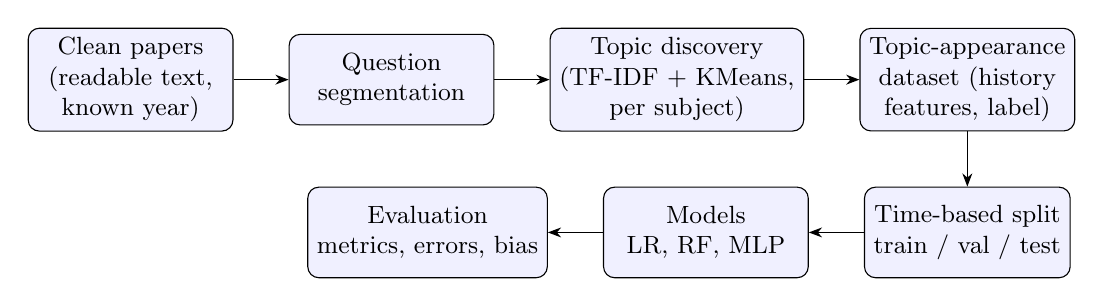
\begin{tikzpicture}[box/.style={draw,rounded corners,align=center,minimum height=1.15cm,minimum width=2.6cm,font=\small,fill=blue!6},
  >=Stealth,node distance=0.7cm]
\node[box] (a) {Clean papers\\(readable text,\\known year)};
\node[box,right=of a] (b) {Question\\segmentation};
\node[box,right=of b] (c) {Topic discovery\\(TF-IDF + KMeans,\\per subject)};
\node[box,right=of c] (d) {Topic-appearance\\dataset (history\\features, label)};
\node[box,below=of d] (e) {Time-based split\\train / val / test};
\node[box,left=of e] (f) {Models\\LR, RF, MLP};
\node[box,left=of f] (g) {Evaluation\\metrics, errors, bias};
\draw[->] (a)--(b); \draw[->] (b)--(c); \draw[->] (c)--(d);
\draw[->] (d)--(e); \draw[->] (e)--(f); \draw[->] (f)--(g);
\end{tikzpicture}}
\caption{Pipeline of Phases 3 and 4. LR = logistic regression, RF = random forest, MLP = multi-layer perceptron.}
\label{fig:pipeline}
\end{figure}

%-------------------------------------------------------------------------------
\section{Problem Formulation and Dataset}
\label{sec:data}

\subsection{Supervised task}
One row of the dataset is a (subject, topic, target exam) triple, where a target exam is a (year, assessment type)
pair of a subject. The label is 1 if at least one paper of that subject, year and type contains a question assigned
to the topic, and 0 otherwise. The model estimates the probability that a topic appears, which fits the uncertainty
argument of the Deliverable~1 AI justification. All features use only papers from strictly earlier years than the
target exam.

\subsection{Question segmentation}
The 1{,}638 clean papers with readable text and a known year (789 quizzes, 532 mids, 317 finals; 105 subjects) are
split into questions by a rule-based segmenter that tries three strategies in order: explicit markers
(\texttt{Question 1}, \texttt{Q2}), numbered items, and a paragraph fallback. Worked solutions, grading tables and
paper-header paragraphs are removed. The result is 7{,}780 questions from 1{,}575 papers (mean 4.9, median 3
per paper): 1{,}001 papers were split on markers, 252 on numbering and 322 by the paragraph fallback. The other 63
papers yielded no question after filtering. Segmentation was checked on random samples and by unit tests, but its
accuracy was not measured against a manually labelled set.

\subsection{Topic discovery}
Topics are discovered per subject, because a topic is only meaningful inside one course. For each subject we fit a
TF-IDF representation (unigrams and bigrams, 2{,}000 features, English and exam-specific stop words) and KMeans
clustering with $K \in [4, 10]$ chosen by cosine silhouette score. Topics are fitted on questions from years up to
2022 only; later questions are assigned to the nearest existing topic, so topic definitions never use future papers.

A subject needs at least 6 papers from at least 3 distinct years and 30 questions in the training period. Of 105
subjects, 28 qualify; 77 are reported as low-confidence and excluded (54 had fewer than 6 training papers, 21 fewer
than 3 training years, one a vocabulary that was too small and one fewer than 30 questions). The 28 subjects have 220
topics (median $K=9$) and 4{,}861 of the 7{,}780 questions (62.5\%) are assigned to a topic. Silhouette scores are low
(median 0.097, range 0.042 to 0.188), as expected for short exam questions with overlapping vocabulary. Most topics
are interpretable (for example ``circuit, switching'' in Computer Networks, ``fitness, chromosome, population'' in
Artificial Intelligence), but some clusters capture generic wording instead of course content.

\subsection{Features}
Table~\ref{tab:features} lists the features. \texttt{years\_since\_last} is missing when a topic has never appeared
before and is imputed on the training split only (Section~\ref{sec:prep}).

\begin{table}[!htb]
\centering
\small
\begin{tabular}{lp{9.0cm}}
\toprule
Feature & Meaning \\
\midrule
\texttt{prior\_papers}, \texttt{prior\_years} & papers and distinct years of the subject before the target year \\
\texttt{topic\_count\_prior}, \trp & appearances of the topic before, and that count divided by \texttt{prior\_papers} \\
\texttt{years\_since\_last} & years since the topic last appeared \\
\texttt{appeared\_last\_year} & 1 if the topic appeared in the year before the target year \\
\texttt{recent\_rate} & appearance rate over the previous two years \\
\texttt{type\_rate\_prior} & appearance rate among earlier papers of the same assessment type \\
\texttt{target\_type} & quiz, mid or final (one-hot encoded) \\
\bottomrule
\end{tabular}
\caption{Model features. A target exam needs at least 3 earlier papers from at least 2 earlier years.}
\label{tab:features}
\end{table}

\subsection{Data split and leakage checks}
\label{sec:split}
The split is by time. Training uses target years 2014 to 2022, validation 2023 and testing 2024 to 2026. The years
were chosen from paper counts before any model was trained. Table~\ref{tab:split} and Figure~\ref{fig:years}
summarise the result.

\begin{table}[!htb]
\centering
\small
\begin{tabular}{lrrrrr}
\toprule
Split & Rows & Positives & Positive rate & Target exams & Subjects \\
\midrule
Train (2014--2022) & 1{,}421 & 672 & 0.473 & 166 & 28 \\
Validation (2023) & 301 & 118 & 0.392 & 36 & 22 \\
Test (2024--2026) & 568 & 197 & 0.347 & 67 & 21 \\
\bottomrule
\end{tabular}
\caption{Size and class balance of each split (2{,}290 rows in total).}
\label{tab:split}
\end{table}

\begin{figure}[!htb]
\centering
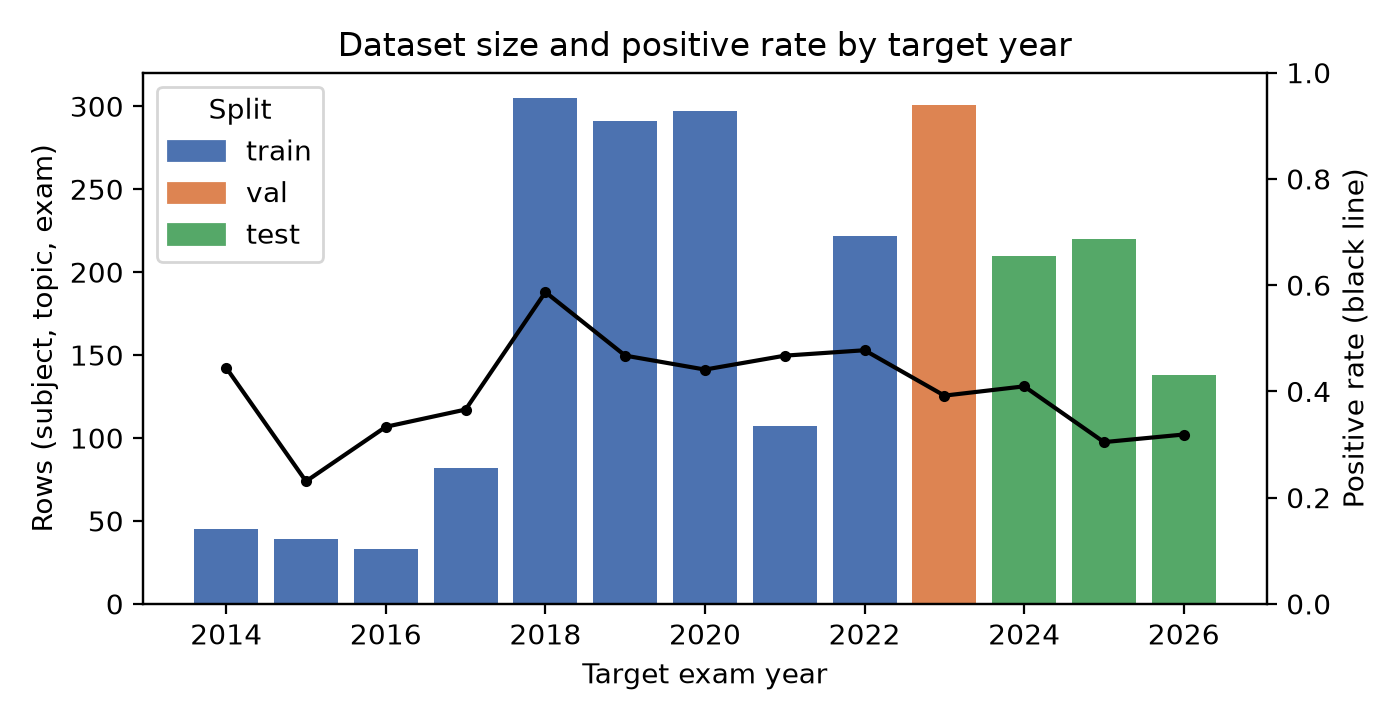
\includegraphics[width=0.85\linewidth]{figures/dataset_by_year.png}
\caption{Rows per target year, coloured by split, with the positive rate (black line).}
\label{fig:years}
\end{figure}

Two checks protect against leakage. A unit test changes only the target-year papers and verifies that every feature
stays identical while the label changes. As a sanity check we also computed the \auc{} of single raw features:
\trp, \texttt{recent\_rate} and \texttt{topic\_count\_prior} reach 0.66 to 0.82 on validation and 0.79 to 0.82 on
test, far below the near-perfect values that a leak would produce. These values also show that a simple frequency
feature is already a strong baseline.

\begin{table}[!htb]
\centering
\small
\begin{tabular}{p{4.0cm}p{2.9cm}p{1.5cm}p{5.7cm}}
\toprule
Data-side setting & Tried & Final & Reason \\
\midrule
Min.\ training papers per subject & 10, 6 & 6 & 10 gave 26 eligible subjects; 6 gave 28 \\
Min.\ training questions & 40, 30 & 30 & enough for stable clustering \\
Min.\ training years & 3 & 3 & recency features need history \\
Topics per subject $K$ & 4 to 10 by silhouette & 4--10 & no single $K$ suits every subject \\
Stop words & English; English + exam + header words & the latter & header words formed meaningless clusters \\
Min.\ prior papers / years per target exam & 3 / 2 & 3 / 2 & history features would be empty \\
Recent window & 2 years & 2 & syllabi change over time \\
\bottomrule
\end{tabular}
\caption{Data-side settings (also in \texttt{docs/data\_settings.md}).}
\label{tab:datasettings}
\end{table}

%-------------------------------------------------------------------------------
\section{Phase 3: Model Architecture and Training}
\label{sec:models}

\subsection{Framework choice}
\label{sec:framework}
We use two industry-standard frameworks. Scikit-Learn 1.9.1 provides logistic regression and a random forest, because
it offers reliable, well-tested implementations and a small, reproducible tuning interface. PyTorch 2.15.0 (CPU) provides
the multi-layer perceptron (MLP), because it gives explicit control over the layers, the loss function, the optimizer
and the training loop (mini-batches, early stopping, restoring the best weights). The code runs on Python 3.14 with a
fixed seed of 42 unless stated otherwise.

\subsection{Preprocessing}
\label{sec:prep}
All preprocessing statistics are fitted on the training split only (1{,}421 rows) and applied unchanged to validation
and test. A unit test checks that changing validation rows does not change any fitted statistic and that no missing
value remains after the transform.
\begin{itemize}
\item \textbf{Missing values.} \texttt{years\_since\_last} is missing for topics never seen before (128 of 1{,}421
training rows). It is filled with the training maximum plus one (10.0), and a binary column \texttt{never\_seen}
marks the filled rows.
\item \textbf{Encoding.} \texttt{target\_type} is one-hot encoded with the categories seen in training (final, mid, quiz).
\item \textbf{Scaling.} The eight numeric features are standardised with the training mean and standard deviation.
\item \textbf{Excluded columns.} Subject, topic id and topic label are not features, so the models cannot memorise
subjects or topics.
\end{itemize}
The result is 12 input features: 8 numeric, 1 indicator and 3 one-hot columns.

\subsection{The models}
Table~\ref{tab:models} lists the learned models. The raw feature \trp{} (the share of earlier papers in which the topic
appeared), used directly as a score without any learning, is an additional reference.

\begin{table}[!htb]
\centering
\small
\begin{tabular}{llp{7.2cm}}
\toprule
Model & Framework & Selected settings \\
\midrule
Logistic regression & Scikit-Learn & $C = 0.01$ \\
Random forest & Scikit-Learn & 300 trees, maximum depth 5, minimum 5 samples per leaf \\
MLP & PyTorch & 12--16--8--1, dropout 0.4, Adam with learning rate 0.01 (Section~\ref{sec:tuning}) \\
\bottomrule
\end{tabular}
\caption{Learned models. All settings were selected on validation \auc{}.}
\label{tab:models}
\end{table}

For logistic regression we tried $C \in \{0.01, 0.1, 1, 10\}$; the validation \auc{} fell slightly from 0.847 to 0.843
as $C$ grew, so stronger regularisation was marginally better. For the random forest we tried 16 settings (trees in
$\{100, 300\}$, maximum depth in $\{3, 5, 8, \text{none}\}$, minimum samples per leaf in $\{1, 5\}$). Validation \auc{}
ranged from 0.789 to 0.827. Forests of unlimited depth with one sample per leaf reached a training \auc{} of 0.99 but the lowest validation \auc{}
(0.79), which is overfitting, so a shallow forest was selected.

\subsection{MLP architecture}
\label{sec:arch}
Figure~\ref{fig:arch} shows the network. It has two hidden layers and a single output unit:
{\small
\[
\text{Linear}(12,16) \rightarrow \text{ReLU} \rightarrow \text{Dropout}(0.4) \rightarrow
\text{Linear}(16,8) \rightarrow \text{ReLU} \rightarrow \text{Dropout}(0.4) \rightarrow \text{Linear}(8,1).
\]}
The selected network has 353 trainable parameters ($12\cdot16+16 + 16\cdot8+8 + 8+1$). The other tested sizes have 961
parameters (32--16) and 2{,}945 parameters (64--32). A small network suits a dataset of 1{,}421 training rows with 12
features.

\begin{figure}[!htb]
\centering
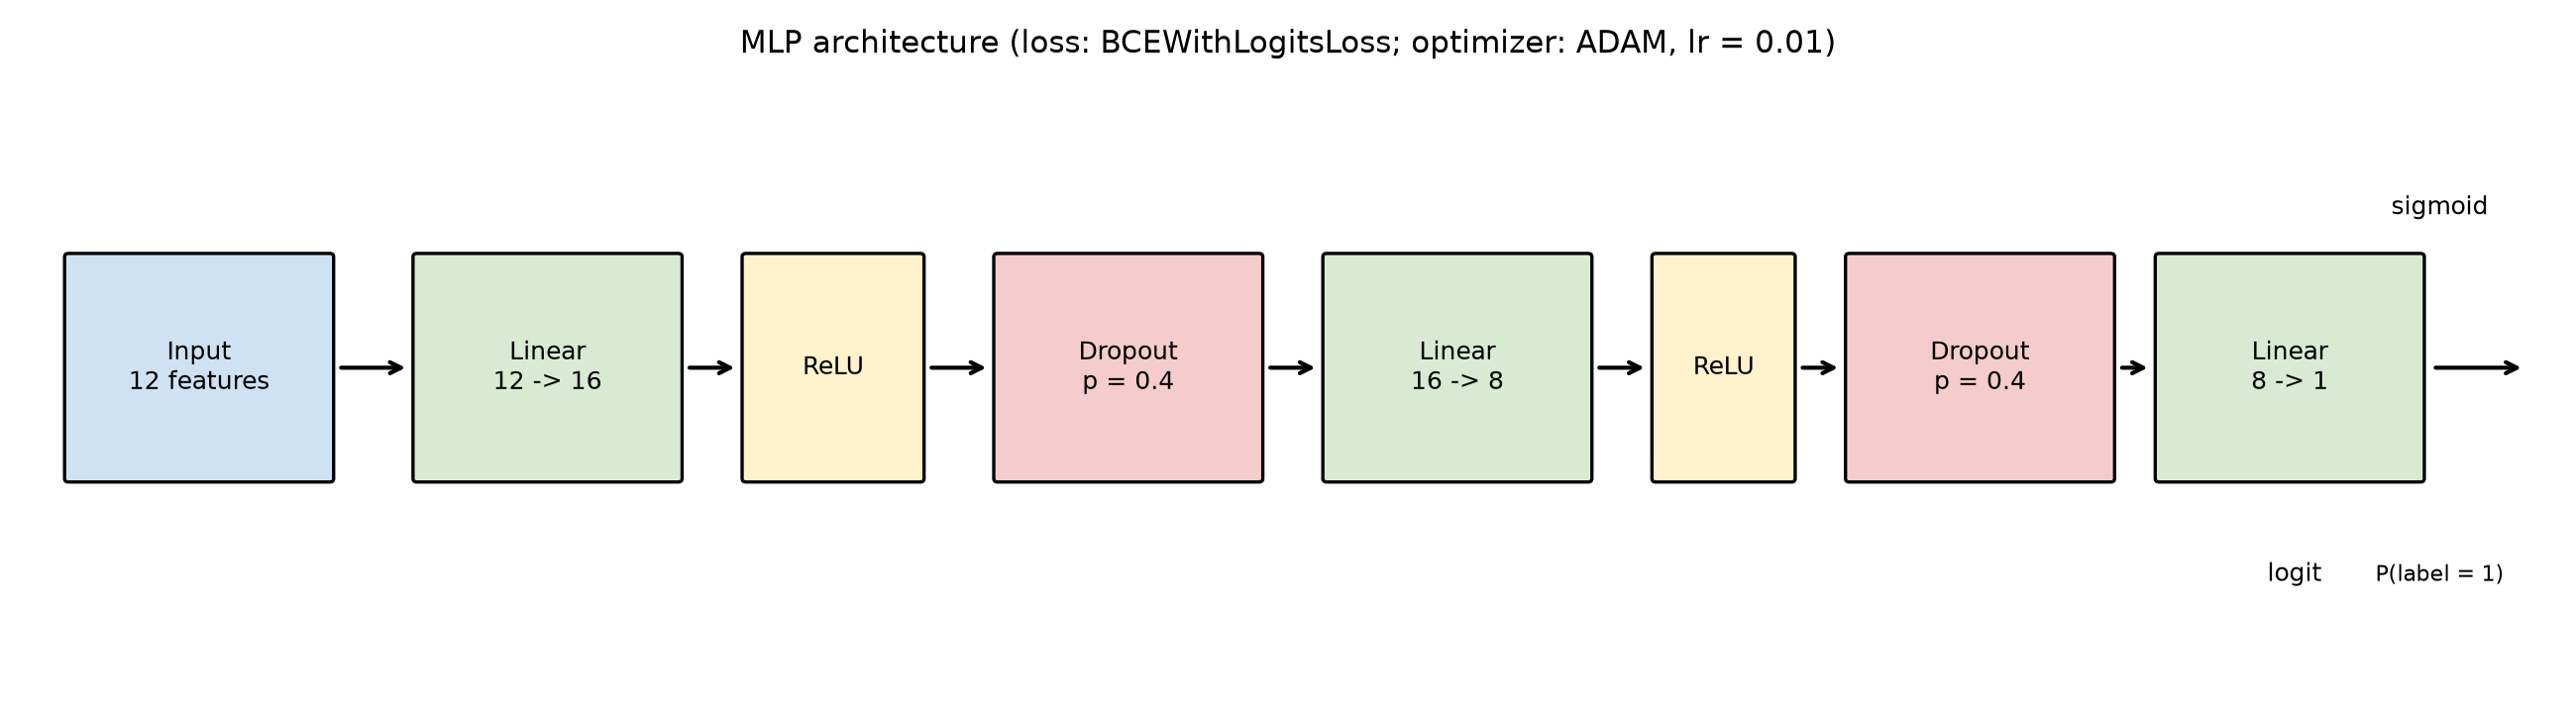
\includegraphics[width=\linewidth]{figures/model_architecture.png}
\caption{Architecture of the final MLP. The network outputs a logit; a sigmoid turns it into the probability that a
topic appears.}
\label{fig:arch}
\end{figure}

\textbf{Layers.} ReLU is a standard, cheap non-linearity. Dropout randomly switches off hidden units during training
as a regulariser. The output is a raw logit; the sigmoid is applied only when probabilities are needed.

\subsection{Loss function and optimizer}
\label{sec:loss}
\textbf{Loss.} We use \texttt{BCEWithLogitsLoss}, which combines the sigmoid and binary cross-entropy in one numerically
stable step and is the natural loss for a binary label with a probability output. The optional \texttt{pos\_weight} is
left off: 47.3\% of training rows are positive, so the weight would be only about 1.11 and the classes are nearly
balanced.

\textbf{Optimizer.} We use Adam with learning rate 0.01, no weight decay and batch size 64. Adam adapts the step size
per parameter and needs little manual tuning. SGD with momentum 0.9 was the alternative in the search.
Training stops early when the validation loss has not improved for 15 epochs (at most 200 epochs), and the weights
of the best epoch are restored.

\subsection{Hyperparameter tuning}
\label{sec:tuning}
We ran a random search over the space in Table~\ref{tab:tuning}, which contains 486 combinations. Forty distinct
configurations were drawn with a fixed seed. Each configuration was trained with three seeds (42, 43, 44) and ranked by
the \emph{mean} validation \auc{} over the three seeds, taken at each run's best validation-loss epoch. The test split
was never loaded during tuning. All 40 results are stored in \texttt{results/tuning\_results.csv}.

\begin{table}[!htb]
\centering
\footnotesize
\begin{tabular}{p{1.8cm}p{2.4cm}p{1.2cm}p{3.2cm}p{5.2cm}}
\toprule
Parameter & Tested values & Final & Mean val.\ \auc{} per value (configs) & Justification \\
\midrule
Learning rate & 0.001, 0.003, 0.01 & 0.01 & 0.8358 (19), 0.8385 (9), 0.8378 (12) & Value of the best configuration; group means differ by less than 0.003. Its best epoch comes after about 10 epochs on average. \\
Batch size & 32, 64, 128 & 64 & 0.8374 (15), 0.8366 (11), 0.8370 (14) & No meaningful difference (range 0.001); 64 is the best configuration's value and gives 23 updates per epoch. \\
Dropout & 0.0, 0.2, 0.4 & 0.4 & 0.8359 (21), 0.8393 (9), 0.8374 (10) & Group means favour 0.2, so 0.4 is not clearly better. Dropout 0.0 had the lowest mean, so some regularisation helps. \\
Hidden sizes & (16,8), (32,16), (64,32) & (16,8) & 0.8363 (10), 0.8356 (12), 0.8384 (18) & Group means slightly favour (64,32); (16,8) is the best configuration and the smallest network (353 parameters). \\
Weight decay & 0, 1e-4, 1e-3 & 0 & 0.8372 (12), 0.8365 (12), 0.8373 (16) & No visible effect, so the simplest setting is kept. \\
Optimizer & Adam, SGD (momentum 0.9) & Adam & 0.8386 (20), 0.8354 (20) & Adam has a slightly higher mean (gap about 0.003) and needs no momentum setting. \\
\bottomrule
\end{tabular}
\caption{Tested hyperparameters, selected values and the mean validation \auc{} over all sampled configurations that used
each value. Fixed: \texttt{pos\_weight} off, patience 15, at most 200 epochs.}
\label{tab:tuning}
\end{table}

The selected configuration (number 35) reached a mean validation \auc{} of 0.8418 with a standard deviation of 0.0026
over the three seeds. The five best configurations lie between 0.8413 and 0.8418, a gap smaller than the seed-to-seed
standard deviation (about 0.002 to 0.003), so the best configuration is only marginally better than its neighbours.
Across all 40 configurations the mean validation \auc{} ranged from 0.822 to 0.842, so architecture and optimizer matter
little on this data. The final configuration is the best single configuration, not a combination of the best value of
each parameter. Because random sampling gave unequal numbers of configurations per value (for example, learning rate
0.001 appears in 19 of 40), the per-value means are descriptive only. Figure~\ref{fig:tuning} shows the 40 results.

\begin{figure}[!htb]
\centering
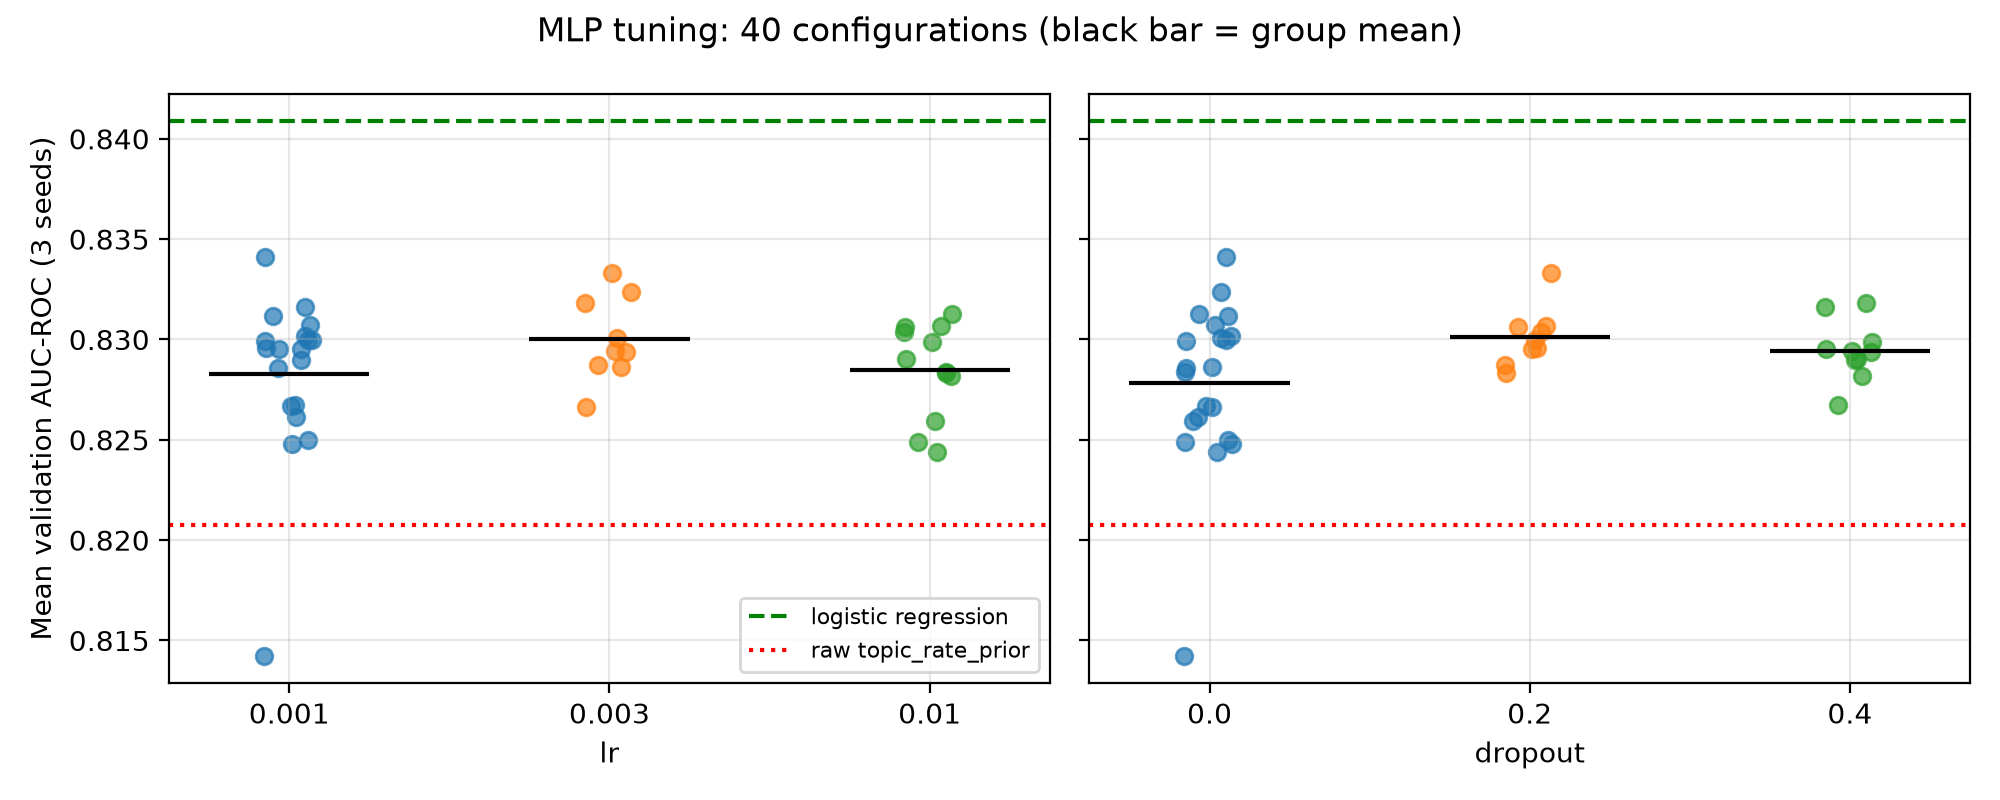
\includegraphics[width=\linewidth]{figures/model_tuning.png}
\caption{Mean validation \auc{} (three seeds) of the 40 tested configurations, grouped by learning rate (left) and
dropout (right). Black bars are group means. The dashed line is logistic regression and the dotted line is the raw
\trp{} feature.}
\label{fig:tuning}
\end{figure}

\subsection{Training curves}
Figure~\ref{fig:curves} shows the loss and accuracy of the final MLP (selected configuration, seed 42). Training
stopped at epoch 24 and the best validation loss (0.5136) occurred at epoch 9, so the weights of epoch 9 are used.
The final run reached a validation \auc{} of 0.838, slightly below the three-seed mean of 0.8418, which is ordinary
seed-to-seed variation.

\begin{figure}[!htb]
\centering
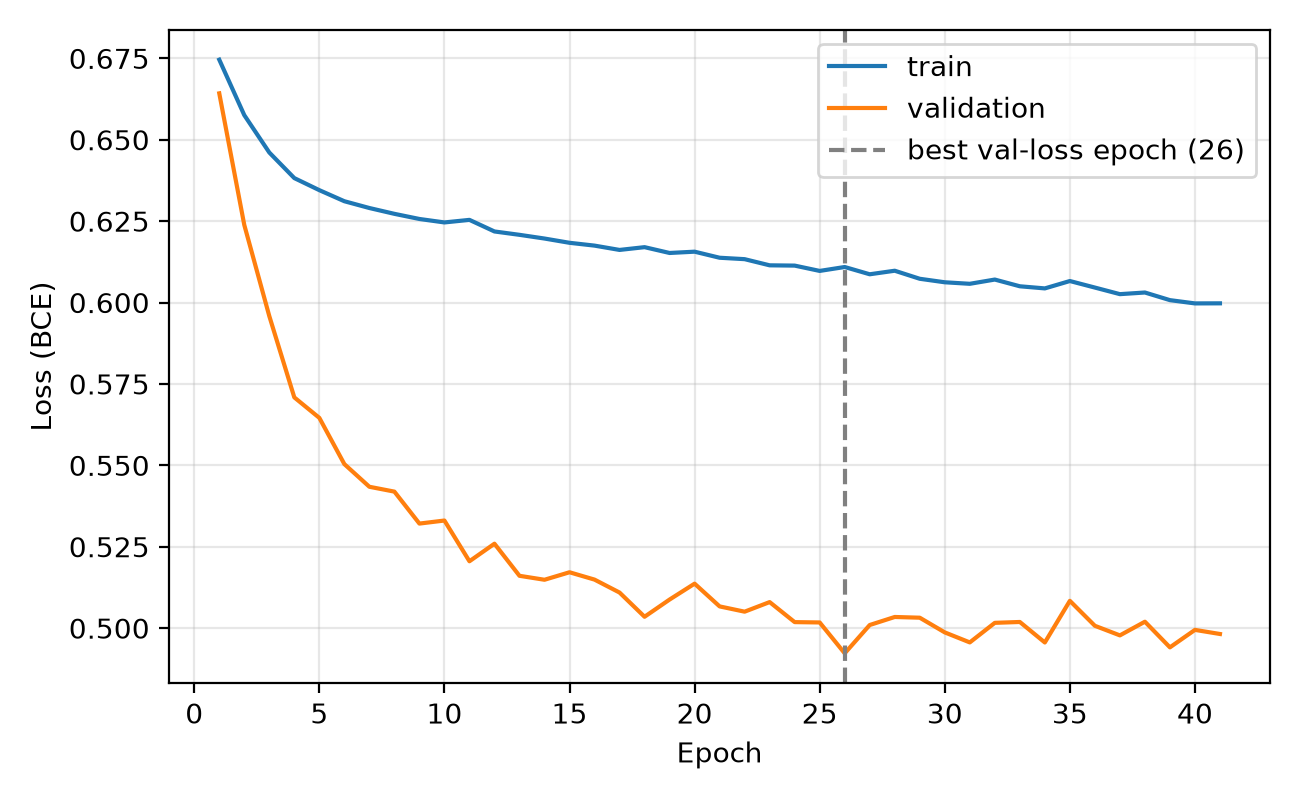
\includegraphics[width=0.49\linewidth]{figures/model_loss_curves.png}\hfill
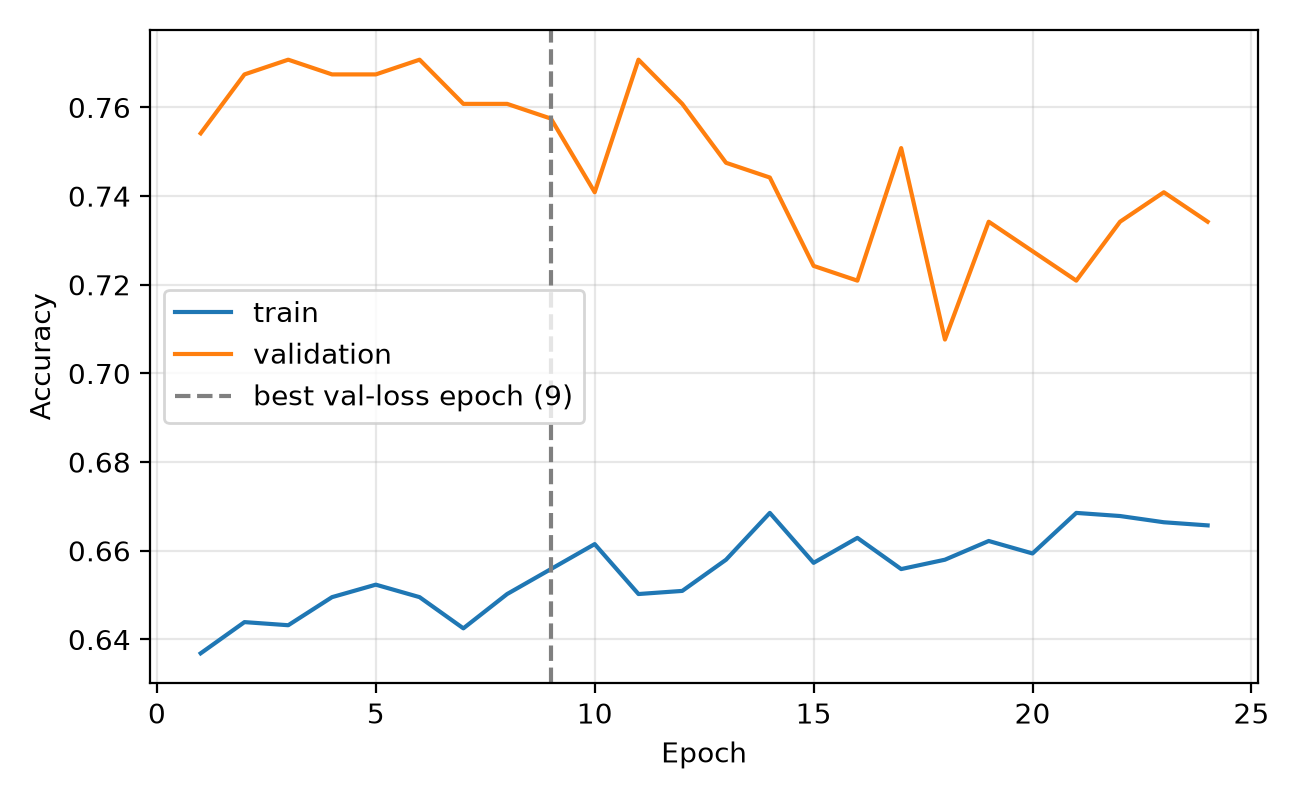
\includegraphics[width=0.49\linewidth]{figures/model_accuracy_curves.png}
\caption{Training and validation loss (left) and accuracy (right) of the final MLP. The dashed line marks the epoch
with the lowest validation loss (epoch 9).}
\label{fig:curves}
\end{figure}

The curves do not show classic overfitting. The training loss decreases slowly, while the validation loss is noisy and
does not improve clearly after epoch 9. Validation accuracy peaks around 0.77 in the first epochs and varies between 0.71 and
0.75 after epoch 13, which supports stopping early. Training accuracy stays between 0.64 and 0.67; for comparison,
always predicting ``does not appear'' would score 0.527 on the training split and 0.608 on validation. The validation
loss is lower than the training loss and validation accuracy is higher than training accuracy. Both are computed with
dropout switched off, so dropout does not explain the gap. A likely reason is that the validation split differs from
the training split: it has a lower positive rate (39.2\% against 47.3\%) and covers only 22 subjects and 36 target
exams. We did not test this explanation, and the gap should not be read as evidence of better generalisation. The modest
training accuracy suggests that the task is hard for these features rather than that the model is too complex.

%-------------------------------------------------------------------------------
\section{Phase 4: Validation and Metrics}
\label{sec:eval}

\subsection{Validation strategy}
\label{sec:validation}
We use a chronological train/validation/test split instead of random K-fold cross-validation. A random split would place
future exams in the training data, so the model would be tested on years it has effectively already seen. It would also
hide the drift of the positive rate over time (47.3\%, 39.2\%, 34.7\%; Table~\ref{tab:split}), and it does not match the
real use, which is to predict an upcoming exam from past ones. The split holds 1{,}421 / 301 / 568 rows (62\% / 13\% /
25\%), and 166 / 36 / 67 target exams. The validation split is the only set used to choose models, hyperparameters and
decision thresholds. The test split is evaluated once, after all models and thresholds were fixed. During tuning, three
seeds per MLP configuration measure the seed-to-seed variation.

\textbf{Decision threshold.} A learned model outputs a probability. The threshold that turns it into a yes/no
prediction is chosen once on validation (maximum F1; ties go to the smallest threshold) and applied unchanged to the
test split. Rule baselines defined by a fixed rule keep that rule as their threshold.

\textbf{Confidence intervals.} Rows of the same target exam (subject, \texttt{target\_year}, \texttt{target\_type}) are
strongly correlated: they share the same papers, and the label depends on which papers the exam group contains. Treating
rows as independent would make intervals too narrow. We therefore resample whole target exams with replacement (1{,}000
resamples, seed 42) and report 95\% percentile intervals. The test split contains only 67 exams and validation only 36,
so small metric differences are within noise. Comparing two intervals of the same exams without pairing is conservative:
overlapping intervals do not prove that two models are equal, only that this data cannot separate them.

\subsection{Metric choice and justification}
\label{sec:metrics}
The classes are roughly balanced but drifting (47.3\% positives in training, 34.7\% in test), so accuracy alone says
little. A student also pays two different costs. A false negative is a topic that appears in the exam but was not
recommended; a false positive is a topic studied for nothing. Accuracy hides this trade-off, so we report:
\begin{itemize}
\item \textbf{Precision}: of the topics we recommend, the share that appear.
\item \textbf{Recall}: of the topics that appear, the share we recommend.
\item \textbf{F1-score}: the harmonic mean of precision and recall; it is also the criterion for the threshold.
\item \textbf{AUC-ROC}: the probability that a random appearing topic is scored above a random non-appearing topic. It
does not depend on a threshold, so it measures ranking quality separately from the threshold choice.
\item \textbf{PR-AUC} (average precision): the area under the precision-recall curve, more informative than \auc{} when
the positive rate differs between splits.
\item \textbf{Brier score}: the mean squared error of the predicted probability (lower is better). It checks calibration,
which matters because the positive rate drifts. It is not reported for scores that are not probabilities (counts) or for
the constant all-positive score.
\end{itemize}

\subsection{Baselines}
Four non-learned baselines show whether learning adds anything over simple rules (Table~\ref{tab:baselines}).

\begin{table}[!htb]
\centering
\small
\begin{tabular}{llp{5.6cm}}
\toprule
Baseline & Threshold & Rule or score \\
\midrule
Rule: count $\geq 5$ & fixed rule & predict 1 if the topic appeared at least 5 times before (the ``appeared 5 times, so
predict it'' rule of the Deliverable~1 AI justification) \\
Rule: appeared last year & fixed rule & predict 1 if the topic appeared in the previous year \\
Raw topic rate & chosen on validation & score = \trp{} \\
All positive & fixed rule & predict 1 for every row \\
\bottomrule
\end{tabular}
\caption{Non-learned baselines.}
\label{tab:baselines}
\end{table}

%-------------------------------------------------------------------------------
\section{Results}
\label{sec:results}

Table~\ref{tab:val} gives the validation results, on which models and thresholds were selected. Table~\ref{tab:testA}
and Table~\ref{tab:testB} give the test results with 95\% cluster-bootstrap intervals.

\begin{table}[!htb]
\centering
\small
\resizebox{\linewidth}{!}{%
\begin{tabular}{lccccccc}
\toprule
Model & Threshold & Precision & Recall & F1 & AUC-ROC & PR-AUC & Brier \\
\midrule
Logistic regression & 0.470 & 0.696 & 0.814 & 0.750 & 0.847 & 0.784 & 0.179 \\
Random forest & 0.470 & 0.640 & 0.814 & 0.716 & 0.827 & 0.742 & 0.174 \\
MLP (PyTorch) & 0.484 & 0.656 & 0.839 & 0.736 & 0.838 & 0.778 & 0.170 \\
\midrule
Rule: count $\geq 5$ & 5.000 & 0.491 & 0.932 & 0.643 & 0.790 & 0.697 & -- \\
Rule: appeared last year & 1.000 & 0.542 & 0.551 & 0.546 & 0.775 & 0.673 & -- \\
Raw topic rate & 0.345 & 0.687 & 0.763 & 0.723 & 0.820 & 0.731 & 0.176 \\
All positive & 1.000 & 0.392 & 1.000 & 0.563 & 0.500 & 0.392 & -- \\
\bottomrule
\end{tabular}}
\caption{Validation results (301 rows, 36 target exams). Thresholds of the learned models and of the raw topic rate
maximise F1 on this split; the other rules keep their fixed threshold. This table is therefore optimistic for them.}
\label{tab:val}
\end{table}

\begin{table}[!htb]
\centering
\small
\begin{tabular}{lccc}
\toprule
Model & Precision & Recall & F1 \\
\midrule
Logistic regression & 0.621 [0.550, 0.688] & 0.766 [0.698, 0.838] & 0.686 [0.632, 0.732] \\
Random forest & 0.595 [0.525, 0.662] & 0.858 [0.800, 0.910] & 0.703 [0.654, 0.745] \\
MLP (PyTorch) & 0.597 [0.525, 0.665] & 0.858 [0.805, 0.913] & 0.704 [0.652, 0.749] \\
\midrule
Rule: count $\geq 5$ & 0.418 [0.363, 0.473] & 0.975 [0.954, 0.991] & 0.585 [0.528, 0.637] \\
Rule: appeared last year & 0.579 [0.511, 0.639] & 0.802 [0.725, 0.868] & 0.672 [0.614, 0.724] \\
Raw topic rate & 0.568 [0.504, 0.631] & 0.655 [0.572, 0.739] & 0.608 [0.560, 0.651] \\
All positive & 0.347 [0.296, 0.398] & 1.000 [1.000, 1.000] & 0.515 [0.457, 0.569] \\
\bottomrule
\end{tabular}
\caption{Test results, threshold-dependent metrics, with 95\% cluster-bootstrap intervals (568 rows, 67 target exams).
Thresholds were fixed on validation.}
\label{tab:testA}
\end{table}

\begin{table}[!htb]
\centering
\small
\begin{tabular}{lccc}
\toprule
Model & AUC-ROC & PR-AUC & Brier score \\
\midrule
Logistic regression & 0.839 [0.796, 0.880] & 0.756 [0.690, 0.819] & 0.173 [0.162, 0.186] \\
Random forest & 0.843 [0.804, 0.881] & 0.741 [0.671, 0.812] & 0.172 [0.160, 0.186] \\
MLP (PyTorch) & 0.849 [0.811, 0.886] & 0.758 [0.694, 0.823] & 0.163 [0.150, 0.178] \\
\midrule
Rule: count $\geq 5$ & 0.822 [0.783, 0.859] & 0.705 [0.641, 0.769] & -- \\
Rule: appeared last year & 0.827 [0.787, 0.865] & 0.713 [0.652, 0.776] & -- \\
Raw topic rate & 0.787 [0.742, 0.830] & 0.688 [0.627, 0.747] & 0.174 [0.152, 0.198] \\
All positive & 0.500 [0.500, 0.500] & 0.347 [0.296, 0.398] & -- \\
\bottomrule
\end{tabular}
\caption{Test results, threshold-free and probability metrics, with 95\% intervals. A constant prediction of the test
positive rate (0.347) would score a Brier value of $0.347 \times 0.653 = 0.227$.}
\label{tab:testB}
\end{table}

\begin{figure}[!htb]
\centering
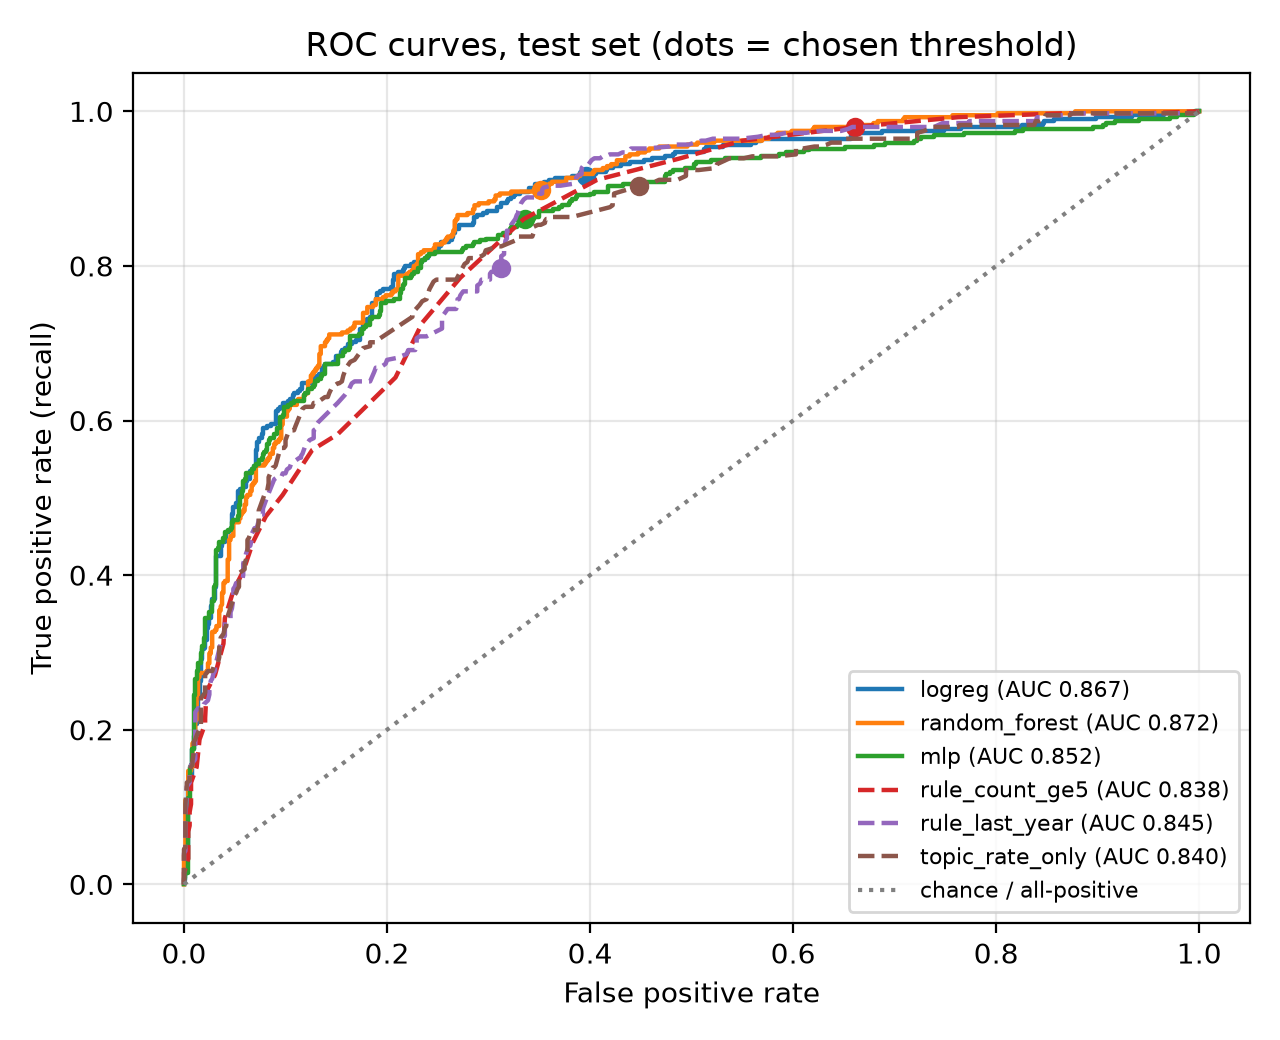
\includegraphics[width=0.48\linewidth]{figures/eval_roc_test.png}\hfill
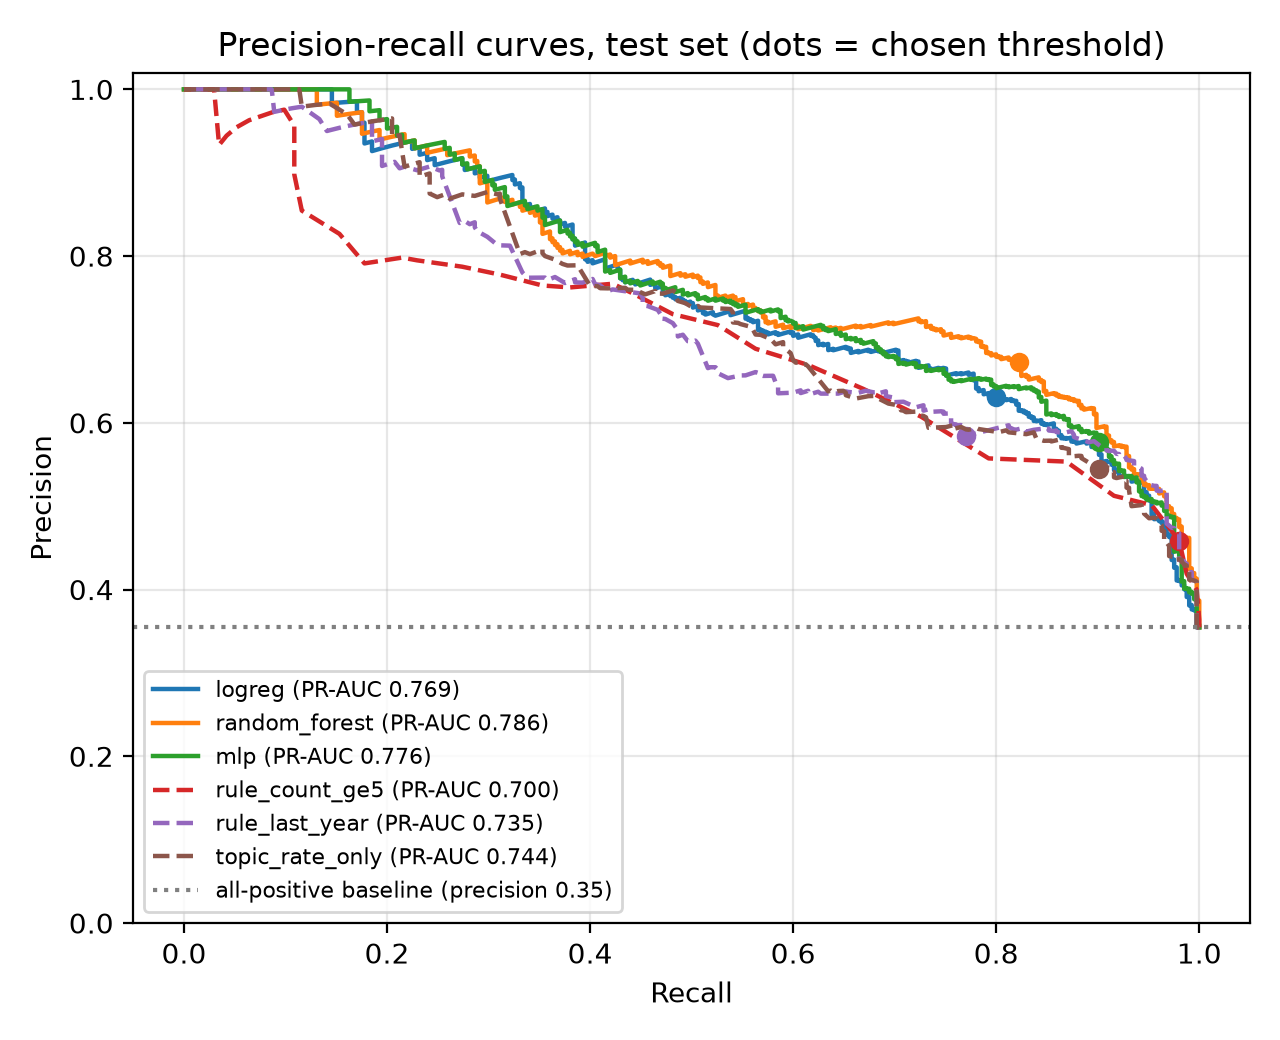
\includegraphics[width=0.48\linewidth]{figures/eval_pr_test.png}
\caption{ROC curves (left) and precision-recall curves (right) on the test split.}
\label{fig:rocpr}
\end{figure}

\begin{figure}[!htb]
\centering
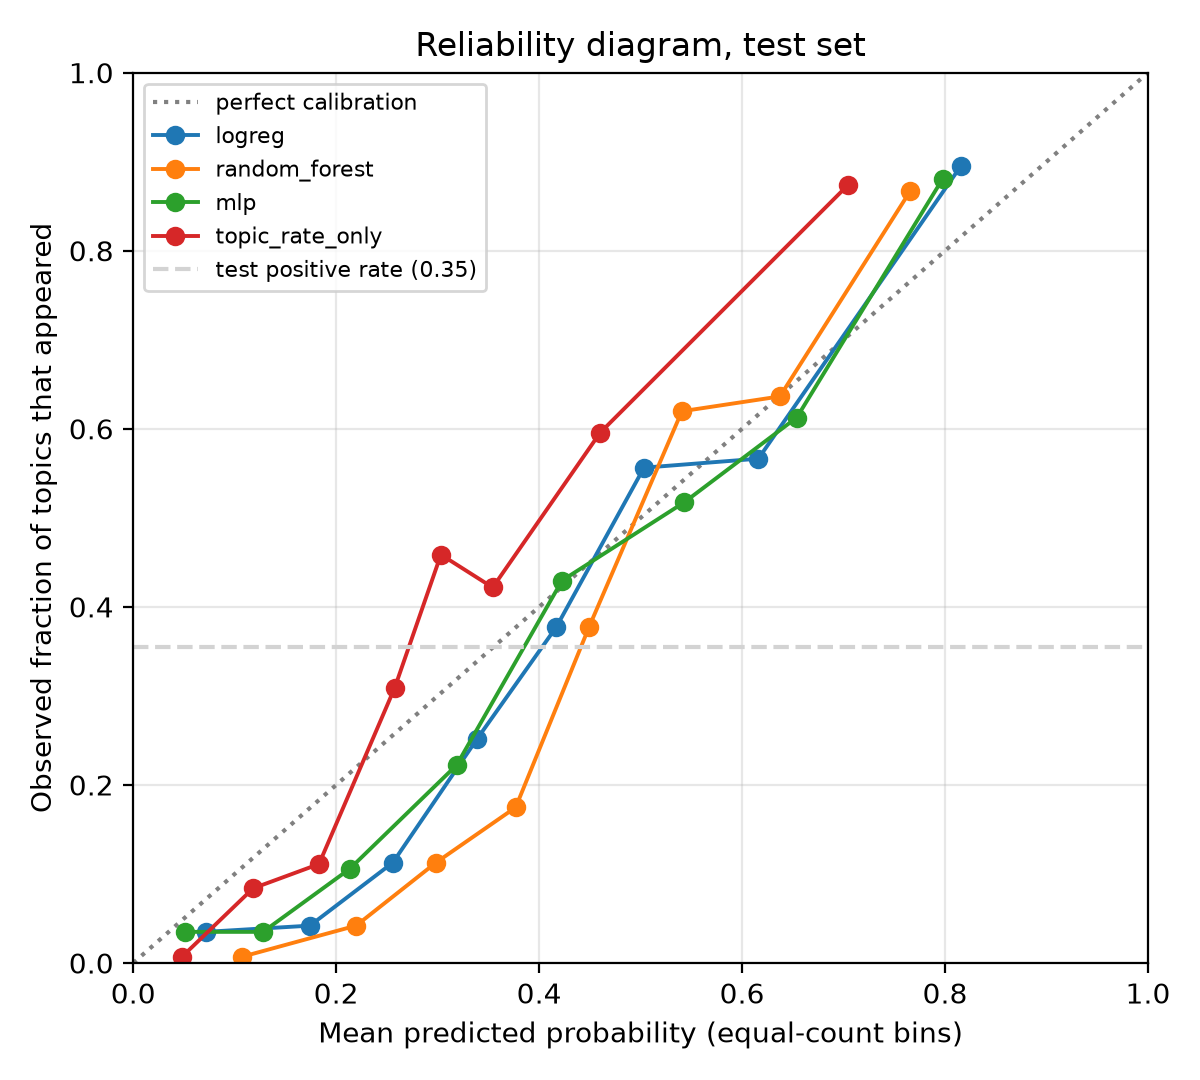
\includegraphics[width=0.62\linewidth]{figures/eval_calibration_test.png}
\caption{Reliability diagram on the test split: mean predicted probability against the observed fraction of topics that appeared.}
\label{fig:cal}
\end{figure}

\begin{figure}[!htb]
\centering
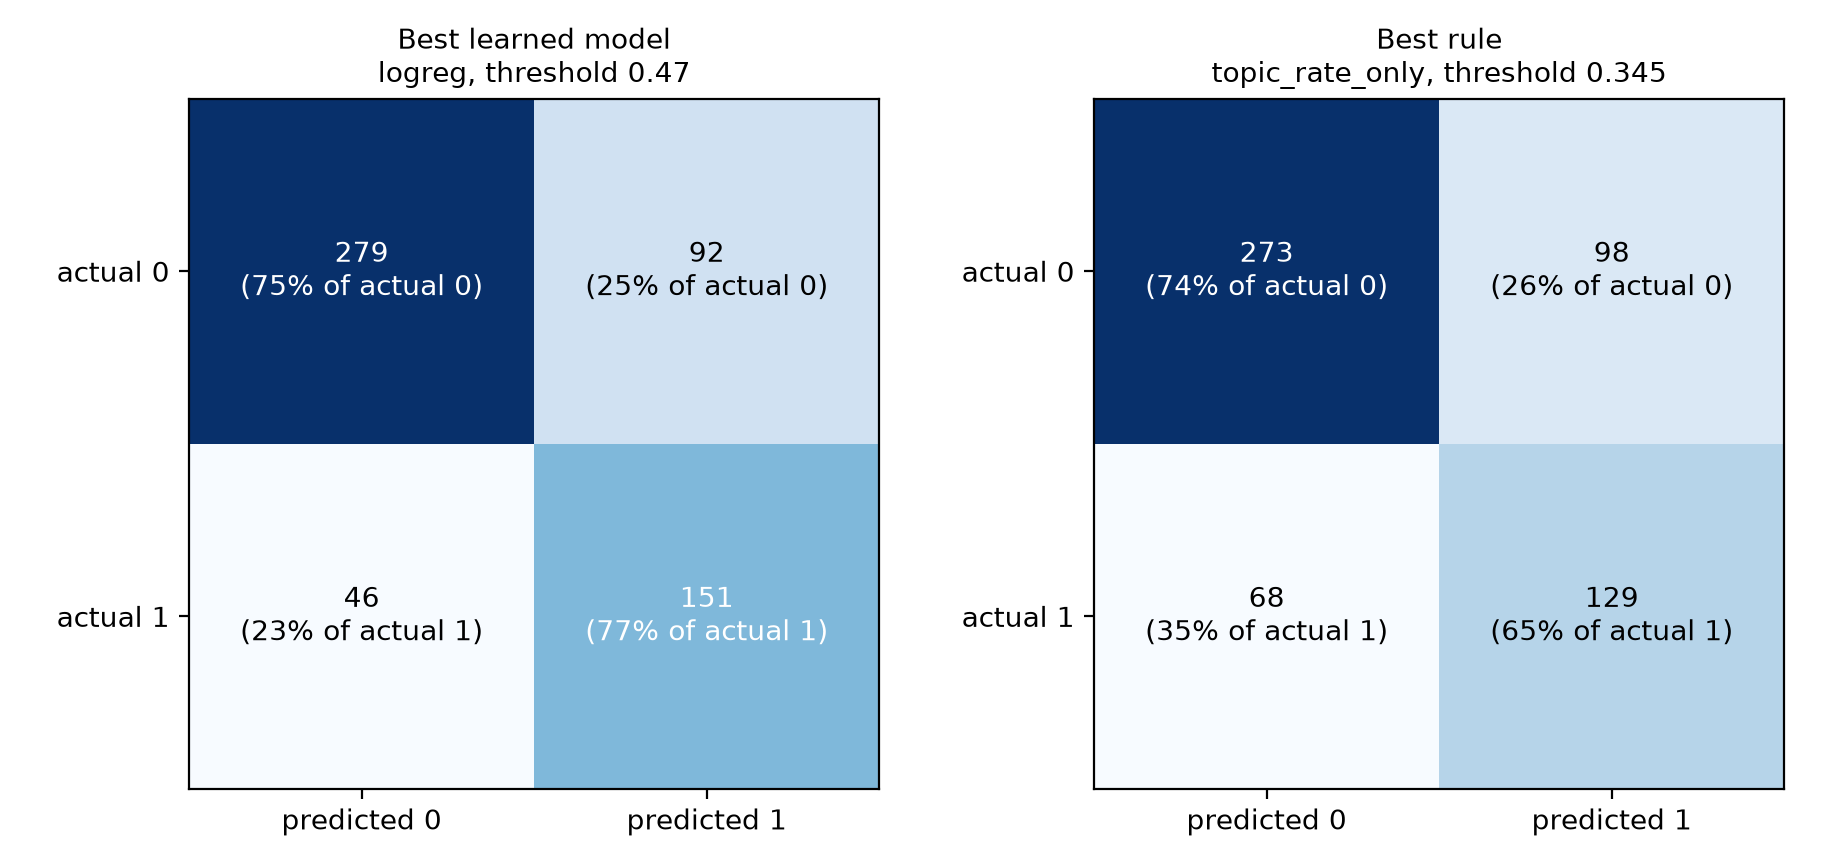
\includegraphics[width=0.95\linewidth]{figures/eval_confusion_test.png}
\caption{Confusion matrices on the test split: the best learned model (logistic regression) and the best rule (raw topic rate).}
\label{fig:conf}
\end{figure}

\subsection{Reading the results}
\textbf{Ranking quality.} On the test split the three learned models reach an \auc{} of 0.839 (logistic regression), 0.843
(random forest) and 0.849 (MLP), with intervals of about $\pm 0.04$ that overlap almost completely. They also overlap with
the history rules: ``appeared last year'' reaches 0.827 and ``count $\geq 5$'' 0.822. The raw topic rate is lowest at
0.787, and even its interval overlaps with those of the learned models. PR-AUC tells the same story. We therefore cannot
claim that any learned model ranks topics better than a one-line rule. The three learned models cannot be told apart
from each other either, which agrees with the tuning results (Section~\ref{sec:tuning}). Only the all-positive
baseline (\auc{} 0.5) is clearly worse.

\textbf{Against the rule of Deliverable 1.} The rule ``appeared at least five times'' flags 459 of 568 test rows (81\%)
as positive. This gives a recall of 0.975 at a precision of only 0.418 (F1 0.585). The learned models flag 43\% to 50\%
of the rows, and their precision (0.595 to 0.621) is clearly higher: the intervals do not overlap. Their recall is
lower (0.766 to 0.858). Their F1 (0.686 to 0.704) is clearly higher for the random forest and the MLP, while the interval
of logistic regression still overlaps that of the rule. One caveat applies: the learned thresholds were tuned on
validation, whereas the rule's threshold of 5 was fixed in advance, so part of this F1 advantage reflects threshold
tuning and not better ranking, which the \auc{} comparison shows to be similar.

\textbf{Against the other baselines.} ``Appeared last year'' cannot be separated from any learned model on any metric
(F1 0.672 against 0.686 to 0.704). The raw topic rate with a validation-tuned threshold reaches an F1 of 0.608 on test; the
intervals of the random forest and the MLP separate from it only narrowly, and the recall of these two models is clearly
higher.

\textbf{Probability quality.} All three learned models beat the constant-rate Brier value of 0.227 (MLP 0.163, random
forest 0.172, logistic regression 0.173), but they overestimate: the mean predicted probability on test is 0.451 (logistic
regression), 0.457 (random forest) and 0.431 (MLP), against an observed rate of 0.347. This matches the drift in the
positive rate. The reliability diagram (Figure~\ref{fig:cal}) shows the overestimate mainly for scores below about 0.55; for
the highest scores the observed fractions are close to the diagonal or above it. Predicted probabilities should be read as
relative rankings, not as calibrated chances.

\textbf{Validation to test.} The \auc{} moved from 0.847 to 0.839 (logistic regression), from 0.827 to 0.843 (random
forest) and from 0.838 to 0.849 (MLP). Selecting on validation therefore did not produce an optimistic gap larger than the
width of the intervals. F1 fell for all three models (for example 0.750 to 0.686 for logistic regression), mainly because
precision fell as the positive rate dropped from 39\% to 35\%.

\textbf{Summary.} The learned models are competitive with, but not demonstrably better than, simple history rules. Their
clearest advantage over the rule of Deliverable~1 is precision: they recommend fewer topics for a similar number of hits.
This is an honest negative result for the claim that machine learning is necessary on this feature set. It does not
settle whether richer, question-level features would change the picture (Section~\ref{sec:limits}).

%-------------------------------------------------------------------------------
\section{Error Analysis}
\label{sec:errors}

We analyse the learned model with the highest validation F1, which is logistic regression (0.750; MLP 0.736, random forest
0.716), at its validation threshold of 0.470. The test split is only broken down here and never used for a choice. On the
test split this model makes 46 false negatives and 92 false positives (151 true positives, 279 true negatives). For each
group Table~\ref{tab:err} gives the numbers of rows and exams, the positive rate, the mean predicted score (a
miscalibration check), precision, recall, F1, \auc{} and the counts of false negatives (FN) and false positives (FP).
Figure~\ref{fig:errgrp} summarises the groups.

\begin{table}[!htb]
\centering
\footnotesize
\resizebox{\linewidth}{!}{%
\begin{tabular}{lrrrrrrrrrr}
\toprule
Group & Rows & Exams & Pos.\ rate & Mean score & Prec. & Rec. & F1 & AUC & FN & FP \\
\midrule
\multicolumn{11}{l}{\emph{Assessment type}} \\
final & 192 & 22 & 0.339 & 0.467 & 0.607 & 0.831 & 0.701 & 0.875 & 11 & 35 \\
mid & 236 & 29 & 0.301 & 0.443 & 0.604 & 0.859 & 0.709 & 0.892 & 10 & 40 \\
quiz & 140 & 16 & 0.436 & 0.442 & 0.679 & 0.590 & 0.632 & 0.734 & 25 & 17 \\
\midrule
\multicolumn{11}{l}{\emph{Target year}} \\
2024 & 210 & 26 & 0.410 & 0.466 & 0.673 & 0.791 & 0.727 & 0.846 & 18 & 33 \\
2025 & 220 & 26 & 0.305 & 0.451 & 0.560 & 0.761 & 0.646 & 0.821 & 16 & 40 \\
2026 & 138 & 15 & 0.319 & 0.427 & 0.627 & 0.727 & 0.674 & 0.846 & 12 & 19 \\
\midrule
\multicolumn{11}{l}{\emph{Earlier papers of the subject}} \\
10-19 & 92 & 13 & 0.293 & 0.472 & 0.667 & 0.963 & 0.788 & 0.946 & 1 & 13 \\
20+ & 476 & 54 & 0.357 & 0.447 & 0.613 & 0.735 & 0.668 & 0.823 & 45 & 79 \\
\midrule
\multicolumn{11}{l}{\emph{Earlier appearances of the topic}} \\
1-2 & 47 & 32 & 0.043 & 0.247 & 0.000 & 0.000 & 0.000 & 0.067 & 2 & 0 \\
3-5 & 114 & 53 & 0.053 & 0.315 & 0.200 & 0.167 & 0.182 & 0.537 & 5 & 4 \\
6+ & 407 & 67 & 0.464 & 0.513 & 0.630 & 0.794 & 0.703 & 0.789 & 39 & 88 \\
\bottomrule
\end{tabular}}
\caption{Test error analysis of logistic regression by group.}
\label{tab:err}
\end{table}

\begin{figure}[!htb]
\centering
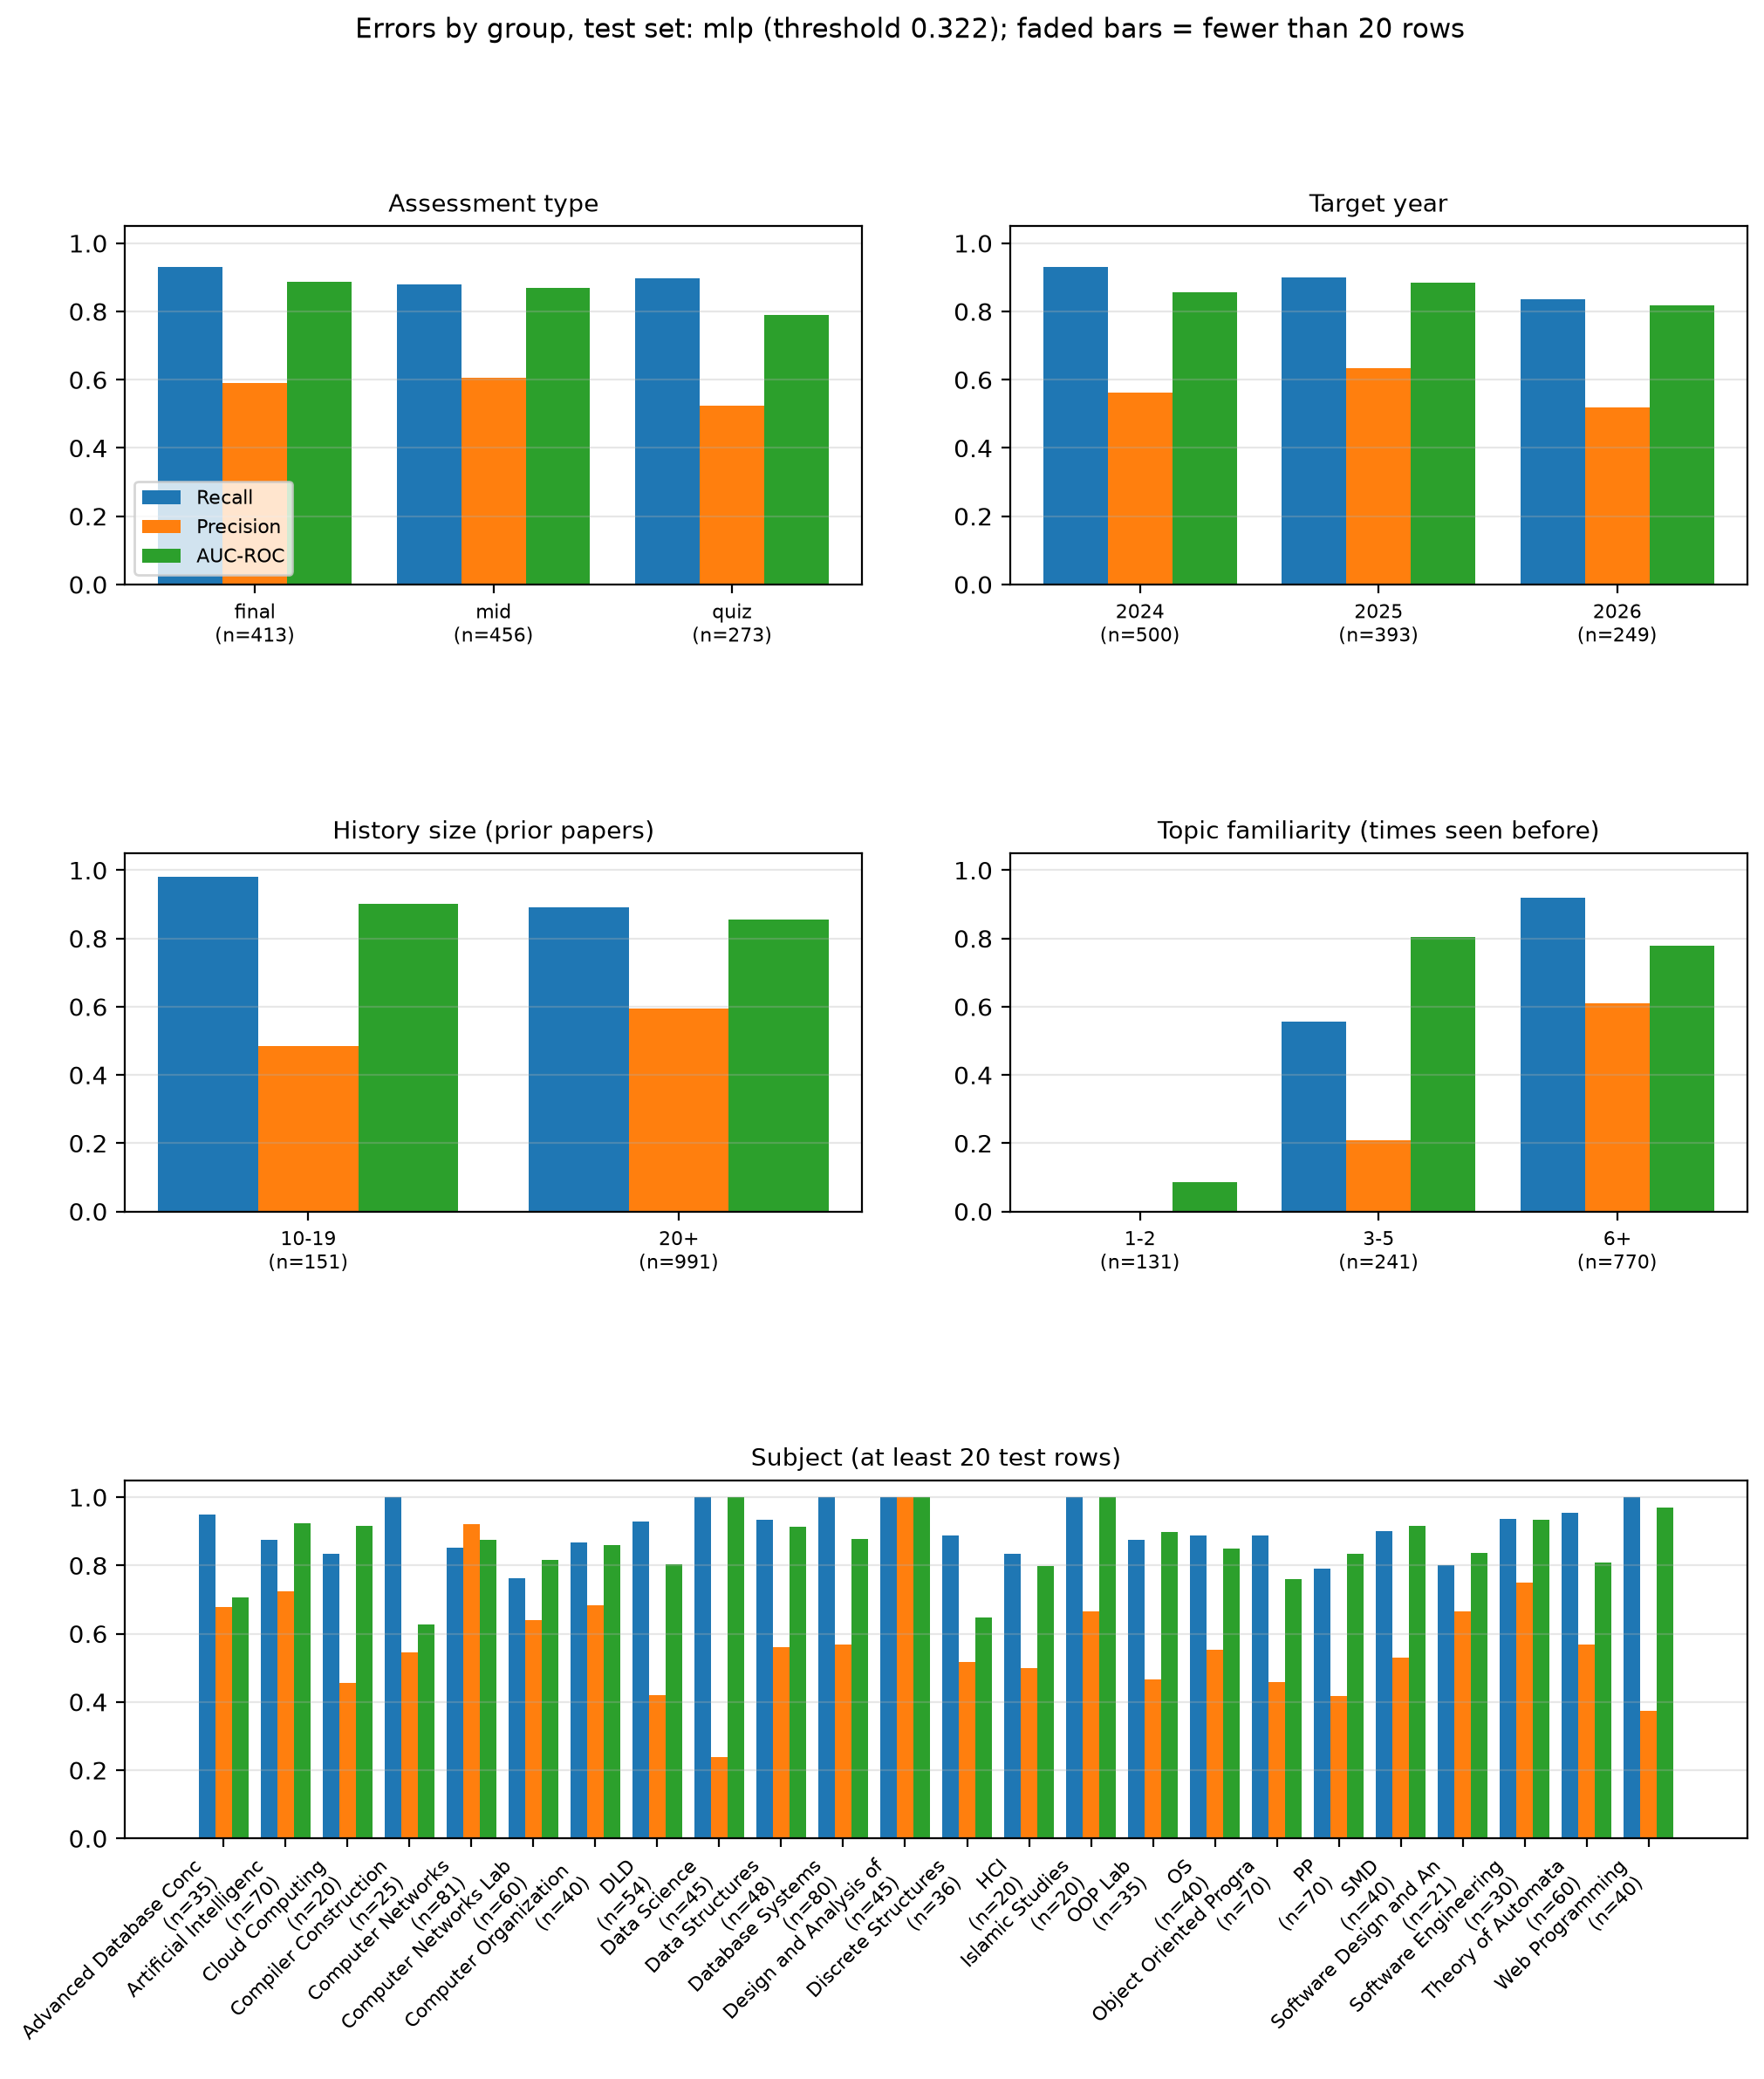
\includegraphics[width=0.92\linewidth]{figures/eval_errors_by_group.png}
\caption{Error analysis by group on the test split.}
\label{fig:errgrp}
\end{figure}

\textbf{Quizzes are the main weakness.} The recall on quizzes is 0.590, against 0.831 for finals and 0.859 for mids, and the
\auc{} is 0.734 against 0.875 and 0.892. Quizzes make up 25\% of the test rows but 25 of the 46 false negatives (54\%).
Quizzes are short (median 2 estimated questions in Deliverable~1), so one quiz covers only a few of a subject's topics. We
did not test whether this explains the gap.

\textbf{Computer Networks is under-predicted.} Table~\ref{tab:subj} shows that Computer Networks has the highest positive
rate (0.588) but a mean score of only 0.405, a recall of 0.574 and a precision of 0.964. It accounts for 20 of the 46 false
negatives (43\%). Topics such as shortest paths, HTTP/TCP and round-trip time are missed most often (Table~\ref{tab:fn}).
The false positives are spread over other subjects (Table~\ref{tab:fp}): PP, Theory of Automata, Database Systems and Design and Analysis of Algorithms.

\begin{table}[!htb]
\centering
\footnotesize
\resizebox{\linewidth}{!}{%
\begin{tabular}{lrrrrrrrrrr}
\toprule
Subject & Rows & Exams & Pos.\ rate & Mean score & Prec. & Rec. & F1 & AUC & FN & FP \\
\midrule
Advanced Database Concepts & 24 & 3 & 0.333 & 0.503 & 0.500 & 1.000 & 0.667 & 0.875 & 0 & 8 \\
Artificial Intelligence & 36 & 4 & 0.444 & 0.495 & 0.750 & 0.938 & 0.833 & 0.872 & 1 & 5 \\
Computer Networks & 80 & 8 & 0.588 & 0.405 & 0.964 & 0.574 & 0.720 & 0.890 & 20 & 1 \\
Data Science & 36 & 4 & 0.111 & 0.424 & 0.571 & 1.000 & 0.727 & 1.000 & 0 & 3 \\
Database Systems & 63 & 7 & 0.429 & 0.495 & 0.649 & 0.889 & 0.750 & 0.874 & 3 & 13 \\
Design and Analysis of Algorithms & 36 & 4 & 0.278 & 0.438 & 0.500 & 0.800 & 0.615 & 0.842 & 2 & 8 \\
Object Oriented Programming & 36 & 4 & 0.306 & 0.355 & 0.667 & 0.545 & 0.600 & 0.851 & 5 & 3 \\
PP & 60 & 6 & 0.233 & 0.460 & 0.400 & 0.714 & 0.513 & 0.859 & 4 & 15 \\
Theory of Automata & 48 & 6 & 0.333 & 0.455 & 0.476 & 0.625 & 0.541 & 0.734 & 6 & 11 \\
Web Programming & 20 & 2 & 0.200 & 0.432 & 0.500 & 0.750 & 0.600 & 0.812 & 1 & 3 \\
\bottomrule
\end{tabular}}
\caption{Test error analysis of logistic regression by subject (subjects with at least 20 test rows; 439 of 568 rows).}
\label{tab:subj}
\end{table}

\begin{table}[!htb]
\centering
\small
\begin{tabular}{p{3.3cm}p{6.6cm}c}
\toprule
Subject & Topic keywords & FN / rows \\
\midrule
Computer Networks & node, algorithm, shortest, paths & 5 / 8 \\
Computer Networks & connection, http, tcp, object & 4 / 8 \\
Computer Networks & transmission round, round, rtt, transmission & 4 / 8 \\
Computer Networks & frame, sends frame, replies frame, replies & 2 / 8 \\
Computer Networks & segment, port, port number, destination port & 2 / 8 \\
Computer Networks & circuit, switching, switched, circuit switching & 2 / 8 \\
Database Systems & customer, number, branch, account & 2 / 7 \\
PP & law, ethics, example, pakistan & 2 / 6 \\
PP & year, rate, years, value & 2 / 6 \\
Theory of Automata & grammar, false, true, context free & 2 / 6 \\
\bottomrule
\end{tabular}
\caption{Topics with the most false negatives (topic keywords come from the clustering).}
\label{tab:fn}
\end{table}

\begin{table}[!htb]
\centering
\small
\begin{tabular}{p{3.3cm}p{6.6cm}c}
\toprule
Subject & Topic keywords & FP / rows \\
\midrule
PP & exam, solve, requirements, framework & 5 / 6 \\
Theory of Automata & initial, deterministic, deterministic finite, finite & 5 / 6 \\
Database Systems & customer, number, branch, account & 4 / 7 \\
Database Systems & update, key, tuple, constraint & 4 / 7 \\
Theory of Automata & dfa, required, nfa, table & 4 / 6 \\
PP & profession, malicious, reasons, information & 3 / 6 \\
PP & law, ethics, example, pakistan & 3 / 6 \\
PP & year, rate, years, value & 3 / 6 \\
Design and Analysis of Algorithms & recurrence, sum, function, left & 3 / 4 \\
Design and Analysis of Algorithms & tree, edge, prove, graph & 3 / 4 \\
\bottomrule
\end{tabular}
\caption{Topics with the most false positives.}
\label{tab:fp}
\end{table}

The same topics appear in both lists in several subjects (for example the PP topics ``law, ethics, example, pakistan'' and
``year, rate, years, value'', and the Database Systems topic ``customer, number, branch, account''), so in
some subjects whether a topic appears in a given exam is only weakly predictable from its history. The most frequent false
positive in PP (5 of 6 rows) is a cluster whose keywords (``exam, solve, requirements, framework'') look like generic wording
rather than syllabus content, which shows how topic noise affects the predictions.

\textbf{Most of the difficulty lies in frequently seen topics.} 407 of the 568 test rows (72\%) are topics that appeared
at least six times before, and 46.4\% of them are positive. The 161 rows of topics seen only one to five times contain only
8 positives (4--5\%), yet the model gives them mean scores of 0.247 and 0.315 (one value per group), so rare topics are overestimated. The model
makes few errors there only because these scores lie below the threshold. The \auc{} of these two groups rests on 2 and 6
positive rows and is not meaningful. Among the frequent topics, which hold 88 of the 92 false positives and 39 of the 46
false negatives, the \auc{} is 0.789, noticeably lower than the overall 0.839. Part of the overall \auc{} therefore comes
from the easy contrast between frequent and rare topics.

\textbf{No cold-start evidence.} The test split contains no topic that never appeared before. All 128 such rows are in
the training split. Performance on entirely new topics, the case where learning could matter most, is therefore not
measured by this evaluation.

\textbf{Years and history.} The \auc{} is 0.846, 0.821 and 0.846 for 2024, 2025 and 2026 and the intervals overlap (Table~\ref{tab:err}),
so we see no trend over time. Precision is lowest in 2025 (0.560), the year with the lowest positive rate (0.305), which agrees
with the drift. Subjects with 20 or more earlier papers have a lower recall (0.735) than subjects with 10 to 19 (0.963), but this
is confounded with the subject, since the large subjects include Computer Networks, and it should not be read as ``more history
hurts''. All test exams have at least 10 earlier papers.

%-------------------------------------------------------------------------------
\section{Bias Check}
\label{sec:bias}

The data contains no demographic attributes: papers are exam sheets, and instructor names are neither reliable nor used
(Deliverable~1). Demographic fairness therefore cannot be assessed. The relevant subgroups are defined by assessment and
data coverage: assessment type, subject coverage tier (small, medium or large by the number of training exams of the
subject, using tertiles), lab versus theory subjects, target year, and amount of history. For each group Table~\ref{tab:bias}
shows recall, precision and \auc{} of the same model as in Section~\ref{sec:errors} with cluster-bootstrap intervals;
Figure~\ref{fig:bias} shows the same comparison graphically.

\begin{table}[!htb]
\centering
\footnotesize
\resizebox{\linewidth}{!}{%
\begin{tabular}{lrrccc}
\toprule
Group & Rows & Exams & Recall & Precision & AUC-ROC \\
\midrule
\multicolumn{6}{l}{\emph{Assessment type}} \\
final & 192 & 22 & 0.831 [0.754, 0.906] & 0.607 [0.495, 0.730] & 0.875 [0.822, 0.925] \\
mid & 236 & 29 & 0.859 [0.779, 0.933] & 0.604 [0.509, 0.696] & 0.892 [0.861, 0.929] \\
quiz & 140 & 16 & 0.590 [0.466, 0.731] & 0.679 [0.521, 0.837] & 0.734 [0.637, 0.839] \\
\midrule
\multicolumn{6}{l}{\emph{Subject coverage tier}} \\
small & 138 & 19 & 0.932 [0.872, 1.000] & 0.631 [0.508, 0.733] & 0.911 [0.857, 0.955] \\
medium & 61 & 8 & 0.909 [0.666, 1.000] & 0.500 [0.300, 0.684] & 0.951 [0.798, 1.000] \\
large & 369 & 40 & 0.704 [0.622, 0.785] & 0.633 [0.543, 0.718] & 0.815 [0.769, 0.862] \\
\midrule
\multicolumn{6}{l}{\emph{Subject kind}} \\
theory & 564 & 66 & 0.765 [0.699, 0.832] & 0.620 [0.553, 0.686] & 0.837 [0.794, 0.877] \\
lab$^{*}$ & 4 & 1 & -- & -- & -- \\
\midrule
\multicolumn{6}{l}{\emph{Target year}} \\
2024 & 210 & 26 & 0.791 [0.701, 0.875] & 0.673 [0.568, 0.774] & 0.846 [0.788, 0.897] \\
2025 & 220 & 26 & 0.761 [0.639, 0.887] & 0.560 [0.452, 0.671] & 0.821 [0.753, 0.898] \\
2026 & 138 & 15 & 0.727 [0.581, 0.892] & 0.627 [0.517, 0.750] & 0.846 [0.746, 0.936] \\
\midrule
\multicolumn{6}{l}{\emph{Earlier papers of the subject}} \\
10-19 & 92 & 13 & 0.963 [0.862, 1.000] & 0.667 [0.514, 0.806] & 0.946 [0.852, 0.994] \\
20+ & 476 & 54 & 0.735 [0.663, 0.808] & 0.613 [0.544, 0.686] & 0.823 [0.779, 0.864] \\
\bottomrule
\end{tabular}}
\caption{Metrics of logistic regression on the test split by subgroup, with 95\% cluster-bootstrap intervals.
$^{*}$Fewer than 20 rows: not reliable, metrics not shown.}
\label{tab:bias}
\end{table}

For each grouping we compare the best and the worst group on four metrics (Table~\ref{tab:gaps}) and call a gap larger than the
uncertainty only if the intervals do not overlap, a conservative test. 4 of the 16 gaps pass it. With
this many comparisons, one or two can appear by chance.

\begin{table}[!htb]
\centering
\footnotesize
\resizebox{\linewidth}{!}{%
\begin{tabular}{llllcc}
\toprule
Grouping & Metric & Best group & Worst group & Gap & Intervals separated \\
\midrule
Assessment type & Recall & mid (0.859) & quiz (0.590) & 0.269 & yes \\
Assessment type & Precision & quiz (0.679) & mid (0.604) & 0.075 & no \\
Assessment type & F1 & mid (0.709) & quiz (0.632) & 0.078 & no \\
Assessment type & AUC-ROC & mid (0.892) & quiz (0.734) & 0.158 & yes \\
\midrule
Subject coverage tier & Recall & small (0.932) & large (0.704) & 0.228 & yes \\
Subject coverage tier & Precision & large (0.633) & medium (0.500) & 0.133 & no \\
Subject coverage tier & F1 & small (0.752) & medium (0.645) & 0.107 & no \\
Subject coverage tier & AUC-ROC & medium (0.951) & large (0.815) & 0.136 & no \\
\midrule
Target year & Recall & 2024 (0.791) & 2026 (0.727) & 0.063 & no \\
Target year & Precision & 2024 (0.673) & 2025 (0.560) & 0.113 & no \\
Target year & F1 & 2024 (0.727) & 2025 (0.646) & 0.082 & no \\
Target year & AUC-ROC & 2024 (0.846) & 2025 (0.821) & 0.025 & no \\
\midrule
Earlier papers of the subject & Recall & 10-19 (0.963) & 20+ (0.735) & 0.228 & yes \\
Earlier papers of the subject & Precision & 10-19 (0.667) & 20+ (0.613) & 0.054 & no \\
Earlier papers of the subject & F1 & 10-19 (0.788) & 20+ (0.668) & 0.119 & no \\
Earlier papers of the subject & AUC-ROC & 10-19 (0.946) & 20+ (0.823) & 0.123 & no \\
\bottomrule
\end{tabular}}
\caption{Largest gap between the best and the worst group, per grouping and metric.}
\label{tab:gaps}
\end{table}


\textbf{Findings.} The clearest gap is assessment type: quizzes have a lower recall than mids and finals and a lower \auc{} than mids. The gaps between the best
group (mids) and the worst (quizzes) exceed the uncertainty for both metrics. Recall also differs by coverage tier (0.932 for small subjects, 0.704 for large ones) and by
history, but the precision and \auc{} gaps are within the uncertainty, so the recall difference may partly be an effect of
the single threshold. Target year shows no separated gap. Lab versus theory cannot be assessed: the test split contains
a single lab exam with 4 rows (all other rows are theory subjects), so the result applies to theory subjects.


\textbf{Data-level bias.} The model can only be as fair as its data. Only 28 of 105 subjects have enough history, so results
do not describe the other 77 subjects, which are reported as low-confidence and receive no prediction. Scanned papers
without extractable text are not spread evenly (Table~\ref{tab:text}): 51.5\% of finals and 44.2\% of mids are unreadable,
against 21.2\% of quizzes. Finals are 23.8\% of the clean papers but only 18.2\% of the readable ones, whereas
quizzes grow from 40.7\% to 50.6\%. The evidence base is therefore thinner for finals. We do not see the
expected consequence in the results: finals perform about as well as mids, and the weakest type is quizzes, the type with the
most readable papers. This does not prove that the scan imbalance is harmless; the cause of the quiz weakness is untested.
Quizzes make up 21.0\% of the training rows, 14.0\% of the validation rows and 24.6\% of the test rows, so they are not
underrepresented in the evaluation data.

\begin{table}[!htb]
\centering
\footnotesize
\resizebox{\linewidth}{!}{%
\begin{tabular}{lrrrrrr}
\toprule
Type & Papers & Readable & Unreadable & Unreadable share & Share of all papers & Share of readable papers \\
\midrule
quiz & 1171 & 923 & 248 & 21.2\% & 40.7\% & 50.6\% \\
mid & 1010 & 564 & 446 & 44.2\% & 35.1\% & 30.9\% \\
final & 684 & 332 & 352 & 51.5\% & 23.8\% & 18.2\% \\
unspecified & 9 & 4 & 5 & 55.6\% & 0.3\% & 0.2\% \\
\midrule
All & 2874 & 1823 & 1051 & 36.6\% & 100\% & 100\% \\
\bottomrule
\end{tabular}}
\caption{Readable text by assessment type among the 2{,}874 clean papers.}
\label{tab:text}
\end{table}


\clearpage
\begin{landscape}
\begin{figure}[H]
\centering
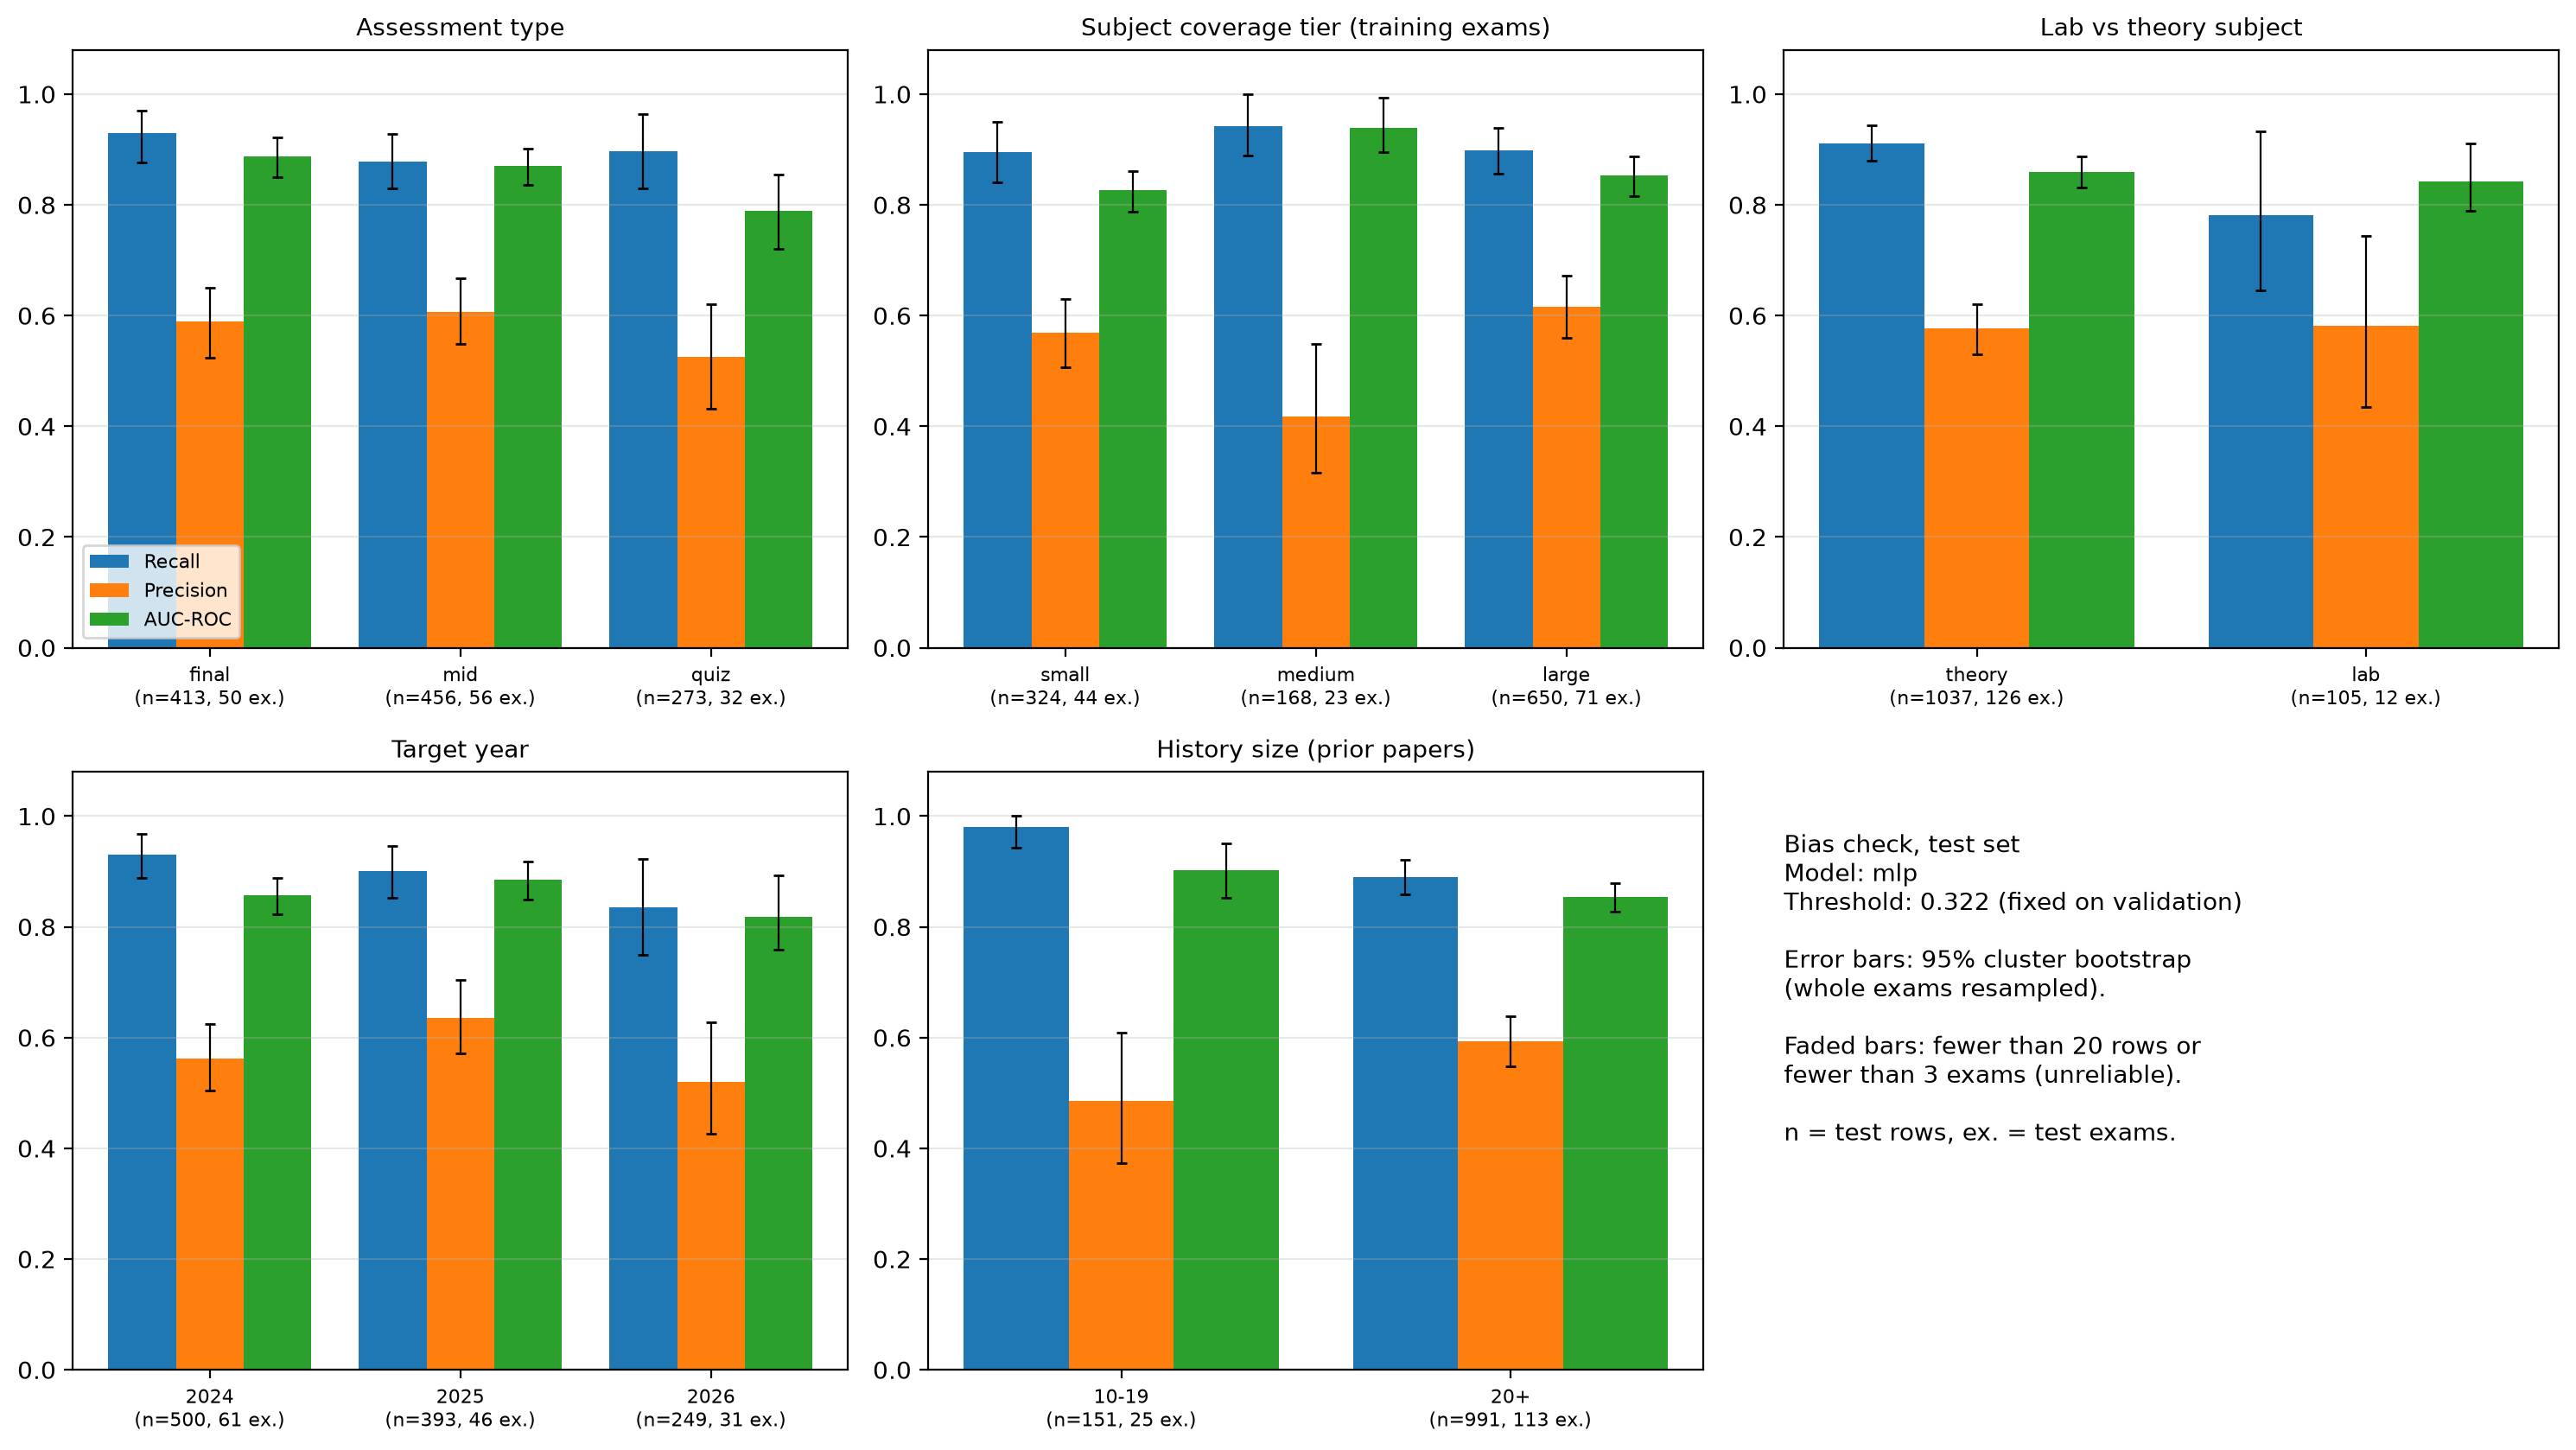
\includegraphics[width=0.97\linewidth]{figures/eval_bias_by_group.png}
\caption{Metrics of logistic regression by subgroup on the test split (error bars: 95\% cluster-bootstrap intervals; faded bars: fewer than 20 rows).}
\label{fig:bias}
\end{figure}
\end{landscape}
\clearpage

%-------------------------------------------------------------------------------
\section{Limitations}
\label{sec:limits}

\begin{itemize}
\item \textbf{Topics are approximate.} They come from unsupervised clustering with low silhouette scores, and some clusters
capture generic wording. Labels inherit this noise. Question-level topic labelling with NLP remains future work.
\item \textbf{The label depends on group size.} An exam group made of several papers (for example Mid~1 and Mid~2 of one year)
has more chances to contain a topic than a single quiz. We do not add group size as a feature because it would use target-year
information.
\item \textbf{Small evaluation sets.} Validation has 36 exams and test 67, so metric differences of a few points are noise, and
the best of 40 tuned configurations is optimistic on validation.
\item \textbf{Distribution drift.} The positive rate falls from 47.3\% to 39.2\% and 34.7\%, and the predicted probabilities
are too high.
\item \textbf{Limited coverage.} 28 of 105 subjects are covered, and the test split contains almost only theory subjects. More than a third of the clean papers
(36.6\%) have no readable text and need OCR, so papers and subjects without readable text are missing.
\item \textbf{No cold-start measurement.} The test split has no never-seen topics, and rare topics have only 8 positives.
\item \textbf{Weak baseline gap.} A one-line history rule is as good as the learned models in ranking, so the benefit of
learning on these features is not demonstrated.
\item \textbf{Metadata and segmentation were checked by sampling, not measured} against a manually labelled set.
\item \textbf{Source quality.} The archive is student-contributed and may contain mislabelled or incomplete papers; it is not
the current syllabus.
\end{itemize}

%-------------------------------------------------------------------------------
\section{Reproducibility, Repository and Model Weights}
\label{sec:repro}

\textbf{Repository.} \url{https://github.com/Minahilbasalat/SpillThePaper}. Phase 3 and 4 code is in \texttt{src/data/} (task,
questions, topics, dataset), \texttt{src/models/} (preprocessing, baselines, MLP, tuning, prediction export) and
\texttt{src/evaluation/} (metrics, baselines, evaluation, error analysis, bias check, contribution table). Tests are in
\texttt{tests/}, committed results in \texttt{results/}, figures in \texttt{report/figures/}, and documentation in
\texttt{docs/}. All work was committed with the Git command line, and every member's commits are listed in
Section~\ref{sec:contrib}.

\textbf{Environment.} \texttt{requirements.txt} lists the dependencies (pandas, matplotlib, seaborn, PyYAML, PyMuPDF,
python-docx, requests, scikit-learn, torch, joblib, pytest). Python 3.14, scikit-learn 1.9.1 and PyTorch 2.15.0 (CPU) were used.
Create a virtual environment, activate it and run \texttt{pip install -r requirements.txt}.

\textbf{Reproduce} (from the repository root, with the environment active; the committed tables in \texttt{data/processed/model/}
are the inputs, so the Deliverable~1 download is not repeated):
\begin{small}
\begin{verbatim}
python -m src.models.baselines
python -m src.models.tune
python -m src.models.train_mlp
python -m src.models.export_predictions
python -m src.models.plots
python -m src.evaluation.baselines
python -m src.evaluation.evaluate
python -m src.evaluation.error_analysis
python -m src.evaluation.bias_check
python -m src.evaluation.contribution_table
python -m pytest tests -q
\end{verbatim}
\end{small}
The data-side scripts (\texttt{src/data/}) need the raw archive of Deliverable~1 and are documented in the README; their
outputs are committed.

\textbf{Model weights.} Weight files are not stored in Git. Following the submission rule, they are hosted externally:
\href{\weightsurl}{Google Drive folder}:
\begin{center}\small\expandafter\url\expandafter{\weightsurl}\end{center}
The folder contains
\texttt{mlp\_best.pt} (the final MLP), \texttt{preprocess.joblib} (the preprocessing fitted on the training split),
\texttt{logreg.joblib} and \texttt{random\_forest.joblib}. The files are small (a few kilobytes for the MLP, about 1.4~MB for
the random forest). They are the outputs of the training scripts above, run on the committed data. All reported metrics are computed from the
committed prediction files in \texttt{results/predictions/}. Re-running the training scripts on a second machine reproduced all six committed prediction files (validation and test, three models) exactly, with a maximum absolute score difference of 0.

%-------------------------------------------------------------------------------
\section{Contribution Table}
\label{sec:contrib}

Table~\ref{tab:contrib} maps Git commit authors to project modules for the Phase 3 and 4 work (commits on \texttt{main}, merge
commits excluded). It was produced from the Git history by \texttt{src/evaluation/\allowbreak contribution\_table.py} after the
code and the evaluation were finished, so the final documentation commits (README and report) are not counted. Author names and e-mail aliases were mapped to the member's real name by
e-mail address. The history contains 60 such commits: 31 by Minahil Basalat, 18 by Khadija Rao and
11 by Iman Abid. A commit that touches several modules counts once for each. ``Python lines'' counts added lines in
\texttt{.py} files of the module.

\begin{table}[!htb]
\centering
\footnotesize
\begin{tabular}{lllrp{6.0cm}}
\toprule
Member & Module & Commits & Python lines & Contents \\
\midrule
\textbf{Minahil Basalat} & \texttt{src/data} & 12 & 674 & schema constants, text loader, question segmenter, topic discovery, dataset builder, dummy-data generator, dataset figure \\
 & \texttt{tests} & 4 & 92 & segmenter tests; leakage test of the dataset builder \\
 & \texttt{docs} & 3 & -- & dataset schema; data-side settings \\
 & \texttt{results} & 6 & -- & Phase 4 outputs (predictions of the rule baselines, metrics, error-analysis and bias tables) produced by the evaluation scripts and committed during integration \\
 & \texttt{report} & 4 & -- & dataset figure; evaluation figures produced by the evaluation scripts, committed during integration \\
 & \texttt{other} & 5 & -- & package skeleton, \texttt{requirements.txt}, \texttt{.gitignore}, README \\
\midrule
\textbf{Khadija Rao} & \texttt{src/models} & 9 & 844 & preprocessing, baselines, MLP, training loop, random search, prediction export, figure generation \\
 & \texttt{tests} & 1 & 137 & preprocessing tests (train-only fitting, no missing values) \\
 & \texttt{docs} & 2 & -- & model documentation and weights link \\
 & \texttt{results} & 5 & -- & baseline and tuning results, MLP training history, predictions of the three learned models \\
 & \texttt{report} & 2 & -- & architecture, training-curve and tuning figures \\
\midrule
\textbf{Iman Abid} & \texttt{src/evaluation} & 9 & 1435 & metrics, cluster bootstrap, predictions contract, rule baselines, evaluation, error analysis, bias check, contribution table \\
 & \texttt{tests} & 1 & 92 & metric tests against hand-computed examples \\
 & \texttt{docs} & 1 & -- & evaluation documentation \\
\bottomrule
\end{tabular}
\caption{Contribution of each member by module (Phase 3 and 4, from the Git history of \texttt{main}).}
\label{tab:contrib}
\end{table}

The \texttt{results} and \texttt{report} rows of the first member record outputs (tables and figures) that the evaluation scripts
generated and that were committed during integration; the code that produced them is in \texttt{src/evaluation}. The
skeleton commit also created empty package files in \texttt{src/models} and \texttt{src/evaluation}. Table~\ref{tab:selected}
lists selected commits for each member.

\begin{table}[!htb]
\centering
\footnotesize
\begin{tabular}{llp{2.6cm}p{6.6cm}}
\toprule
Author & Commit & Module & Message \\
\midrule
Minahil Basalat & \texttt{ed0e3ac} & \texttt{src/data} & feat(data): add loader that joins papers\_clean with extracted text \\
Minahil Basalat & \texttt{268874c} & \texttt{src/data} & feat(data): add rule-based question segmenter with marker, numbered and paragraph fallbacks \\
Minahil Basalat & \texttt{0135a7a} & \texttt{data files, src/data} & feat(data): per-subject topic discovery (TF-IDF + KMeans) fitted on train years only \\
Minahil Basalat & \texttt{c83ce19} & \texttt{src/data} & feat(data): add leakage-safe topic-appearance dataset builder with time-based split \\
Minahil Basalat & \texttt{0334616} & \texttt{tests} & test(data): verify dataset features use only earlier years (leakage test) \\
Khadija Rao & \texttt{ce3d232} & \texttt{src/models} & feat(models): add train-only preprocessing (imputation, one-hot, scaling) \\
Khadija Rao & \texttt{3be7d1a} & \texttt{src/models} & feat(models): add logistic regression and random forest baselines tuned on val AUC \\
Khadija Rao & \texttt{b947601} & \texttt{src/models} & feat(models): add PyTorch MLP with BCEWithLogits loss and Adam/SGD options \\
Khadija Rao & \texttt{87de66c} & \texttt{src/models} & feat(models): add random search over MLP hyperparameters (40 configs x 3 seeds) \\
Khadija Rao & \texttt{d6516d1} & \texttt{src/models} & feat(models): add MLP training loop with early stopping and history logging \\
Iman Abid & \texttt{b15d35e} & \texttt{src/evaluation} & feat(evaluation): add metrics, F1 threshold selection and cluster bootstrap \\
Iman Abid & \texttt{b42fdb9} & \texttt{src/evaluation} & feat(evaluation): add rule-based baselines in the shared predictions format \\
Iman Abid & \texttt{a8e4b7f} & \texttt{src/evaluation} & feat(evaluation): add evaluate script with val-chosen threshold and cluster-bootstrap CIs \\
Iman Abid & \texttt{0954390} & \texttt{src/evaluation} & feat(evaluation): add error analysis by group with top false negatives and positives \\
Iman Abid & \texttt{5dab161} & \texttt{src/evaluation} & feat(evaluation): add bias check across assessment, coverage, lab/theory, year and history groups \\
\bottomrule
\end{tabular}
\caption{Selected commits (full history: \texttt{results/contribution\_commits.csv}).}
\label{tab:selected}
\end{table}

%-------------------------------------------------------------------------------
\section{Conclusion}
\label{sec:concl}

We turned an unlabelled archive of exam papers into a supervised, leakage-safe task, trained three models with documented
tuning, and evaluated them chronologically with confidence intervals, error analysis and a bias check. The learned models
rank topics with an \auc{} of about 0.84 to 0.85 and are clearly more precise than the ``appeared five times'' rule of
Deliverable~1, but they are not demonstrably better than ``appeared last year''. They are weakest on quizzes and on
Computer Networks, overestimate probabilities, and cannot be evaluated on topics never seen before. The main next steps are
OCR for the 36.6\% of clean papers without readable text, question-level topic labelling with NLP and comparison with the current syllabus,
a model that tolerates the missing cold-start case, and, in later phases, the tentative paper generator and the personalised
practice.

\end{document}